\documentclass[paper=a4, fontsize=12pt]{scrartcl} % A4 paper and 11pt font size

\usepackage[T1]{fontenc} % Use 8-bit encoding that has 256 glyphs
%\usepackage{fourier} % Use the Adobe Utopia font for the document - comment this line to return to the LaTeX default
\usepackage[english]{babel}
\usepackage{amsmath} % Math packages
\usepackage{amsfonts}
\usepackage{amsthm}
\usepackage{afterpage}
\usepackage{lipsum} % Used for inserting dummy 'Lorem ipsum' text into the template
\usepackage{listings}
\usepackage{rotating}
\usepackage{graphicx}
\usepackage{sectsty} % Allows customizing section commands
\usepackage{fancyhdr}
\usepackage{xcolor}
\usepackage{multirow}
\usepackage[nottoc]{tocbibind}
\allsectionsfont{\centering \normalfont\scshape} % Make all sections centered, the default font and small caps
\usepackage{fancyhdr} % Custom headers and footers
\pagestyle{fancyplain} % Makes all pages in the document conform to the custom headers and footers
\fancyhead{} % No page header - if you want one, create it in the same way as the footers below
\fancyfoot[L]{} % Empty left footer
\fancyfoot[C]{} % Empty center footer
\fancyfoot[R]{\thepage} % Page numbering for right footer
\renewcommand{\headrulewidth}{0pt} % Remove header underlines
\renewcommand{\footrulewidth}{0pt} % Remove footer underlines
\setlength{\headheight}{13.6pt} % Customize the height of the header
\setlength\parindent{0pt} % Removes all indentation from paragraphs - comment this line for an assignment with lots of text
\numberwithin{equation}{section}

\newcommand\blankpage{%
    \null
    \thispagestyle{empty}%
    \addtocounter{page}{-1}%
    \newpage}
    

\makeatletter
\newcommand{\distas}[1]{\mathbin{\overset{#1}{\kern\z@\sim}}}%
\newsavebox{\mybox}\newsavebox{\mysim}
\newcommand{\distras}[1]{%
  \savebox{\mybox}{\hbox{\kern3pt$\scriptstyle#1$\kern3pt}}%
  \savebox{\mysim}{\hbox{$\sim$}}%
  \mathbin{\overset{#1}{\kern\z@\resizebox{\wd\mybox}{\ht\mysim}{$\sim$}}}%
}
\makeatother

\makeatletter
\renewcommand\paragraph{\@startsection{paragraph}{4}{\z@}%
            {-2.5ex\@plus -1ex \@minus -.25ex}%
            {1.25ex \@plus .25ex}%
            {\normalfont\normalsize\bfseries}}
\makeatother
\setcounter{secnumdepth}{4} % how many sectioning levels to assign numbers to
\setcounter{tocdepth}{4}    % how many sectioning levels to show in ToC



\usepackage{listings}
\usepackage{color}
\definecolor{dkgreen}{rgb}{0,0.6,0}
\definecolor{gray}{rgb}{0.5,0.5,0.5}
\definecolor{mauve}{rgb}{0.58,0,0.82}

\lstset{frame=tb,
  language=R,
  aboveskip=3mm,
  belowskip=3mm,
  showstringspaces=false,
  columns=flexible,
  basicstyle={\small\ttfamily},
  numbers=none,
  numberstyle=\tiny\color{gray},
  keywordstyle=\color{blue},
  commentstyle=\color{dkgreen},
  stringstyle=\color{mauve},
  breaklines=true,
  breakatwhitespace=true,
  tabsize=3
}



%----------------------------------------------------------------------------------------
%	TITLE SECTION
%----------------------------------------------------------------------------------------

\newcommand{\horrule}[1]{\rule{\linewidth}{#1}} % Create horizontal rule command with 1 argument of height

\fancyhf{}% Clear all headers/footers
\fancyhead[L]{Master Thesis}\fancyhead[C]{}\fancyhead[R]{Alessandro Bellotta}
\fancyfoot[L]{USI - Universit� della Svizzera Italiana, MSc in Finance}\fancyfoot[C]{}\fancyfoot[R]{\thepage}
\pagestyle{fancy}
\thispagestyle{plain}
\renewcommand{\headrulewidth}{0.4pt}
\renewcommand{\footrulewidth}{0.4pt}

\title{	
\normalfont \normalsize 
\textsc{USI - Universit� della Svizzera Italiana, Lugano} \\ % Your university, school and/or department name(s)
\textsc{Facolt� di Scienze Economiche}\\
\textsc{MSc in Finance} \\[100pt]
\textsc{Master Thesis}\\ [50pt]
\horrule{2pt} \\[0.5cm] % Thin top horizontal rule
\huge Option Pricing with Stochastic Volatility, Jumps and Fractals Processes \\ % The assignment title
\horrule{2pt} \\[0.5cm] % Thick bottom horizontal rule
}
\author{Alessandro Bellotta\\
{\small Supervised by: Prof. Patrick Gagliardini, PhD}\\
{\small Second Reader: Prof. Paul Schneider, PhD}}
\date{February 2017} 

\begin{document}

\maketitle \thispagestyle{empty}% Print the title

\afterpage{\blankpage}
\newpage  \thispagestyle{empty}

%------------------------
% CITATION
%------------------------	
	\section*{} 
	\begin{flushright}
		\textit{And in the end, it's not the years in your life that count. It's the life in your years.\\ - Abraham Lincoln} 
	\end{flushright}
\afterpage{\blankpage}
\newpage \thispagestyle{empty}
%------------------------
% DEDICATE TO
%------------------------	
	\section*{}
	\begin{flushright}
		\textit{Dedicated to my mother, my father and Laura}
	\end{flushright}
\afterpage{\blankpage}
\newpage

%--------------	TABLE OF CONTENT ---------------
\tableofcontents
%\afterpage{\null\newpage}
\newpage 
\listoffigures
\newpage 
\lstlistoflistings
\listoftables

\afterpage{\pagestyle{empty}
\newpage~\newpage~\newpage}
\newpage
%------------------------
% ABSTRACT
%------------------------	
\section{Abstract}
The aim of this thesis is to develop a broad analysis on option pricing models such as Black-Scholes model, Heston stochastic volatility model and jump-diffusion model. \par
In addition we want also to analyse a non-ordinary theory that is called Fractal Market Hypothesis in which we also price options with, the so-called, Fractal Brownian Motion. \par
What we want to show is a computational approach to this field: we start from theoretical and mathematical formulations and then we apply IT models in order to implement the theory; the choosen software is R.	\par
The aim is not only to plug-in numbers in already-built function but also to develop step-by-step the theory and then to create algorithms to achieve the task (pricing) that are calibrated on real-world data and that are able to adapt when another input is chosen.	\par
What we are calling pricing, is, for the sake of preciseness, a computation of future expected values; starting from this concept, an investor could implement its own strategy. 

\afterpage{\blankpage}
\newpage

%------------------------
%INTRODUCTION
%------------------------
\section{Introduction}
This paragraph is aimed to introduce the following work.	\par
What we want to achieve is both an academic and practical analysis and, in addition, a not-so-conventional approach to a fundamental financial field.	\par
Our objective is to deliver a broad analysis about option pricing and to analyse something that is not mainstream and widespread.	\par
First we want to present models from the theory and from a mathematical perspective. In order to achieve this goal, we will deliver a broad but concise analysis of models: model formulation, useful mathematics, properties and derivation. \par
In a second step, we explain what was done in order to implement the theory with a computational approach: here, we explain formulae, methodologies, calibration and results that we get.	\par
In the third step we provide code chunks that are useful in order to understand how the analysis evolved.	\par
How is this thesis built? \par
First of all we define an option: to be more precise, in this thesis we deal with European Call Option. \par
Then, we start with models: the Black-Scholes model, the Heston model, the jump-diffusion model.\par
In the end we analyse the Fractal Market Hypothesis as an alternative to the Efficient Market Hypothesis: in order to do this we first define "fractal" with some examples, then we perform a "Rescaled Range Analysis" that aims to find the famous Hurst Exponent ($H$) and, in the end, we price a call option by applying fractal Brownian motion.	\par
In addition, we deliver an analysis in a Monte Carlo framework and an appendix with mathematics useful for this work.

\afterpage{\blankpage}
\newpage

%------------------------
% OPTION: BASIC CONCEPTS
%------------------------
\section{Options: Basic Concepts}
		
%---------	WHAT IS AN OPTION?	--------------
\subsection{What is an Option?}
A derivative asset can be defined as a financial instrument whose value depends on the value of other underlying variables. The variables underlying derivatives can belong to different asset classes such as traded securities, interest rates, volatility and so on. \par
There exist two big classes of options: call options and put options. \par
From this dichotomy, we can analyse whether the position is long or short: it is long when the investor has bought the option; it is short when the investor has written the option.
A call option gives the holder the right to buy an asset by a certain date (maturity date, $T$) for a certain price (strike price, $K$). The payoff at maturity is:\par
	\begin{equation}	
		call \hspace{0.2cm} payoff = \max(S_{T}-K, 0)	 	
	\end{equation}
Where $S_T$ is the underlying price at maturity and $K$ is the strike price.
A Put option is an arrangement which allows to sell shares of the underlying at an agreed price in a particular date. \par
	\begin{equation}	
		put \hspace{0.2cm} payoff = \max(K-S_{T}, 0)
	\end{equation}


In this thesis, we will analyse a specific type of option: European call option. It is called in this way because it can be exercised only at maturity (European type). In order to be consistent, in the appendix we will provide a proof of the put-call parity in order to show that, once priced a call, it is possible to get to the put value through a mathematical formula. \par
When we deal with pricing, we must take into account some variables; in addition to the over mentioned $S$ and $K$ we have: $\tau$ which is the time to maturity, $\sigma$ which is the volatility of the underlying and $r$ which is the risk-free rate. Then, $C$ is the value of a call option which depends on all these variables.	\par

Once defined the option payoff, it is possible to show that the price of the option can be represented as a conditional expectation of the payoff under the risk-neutral measure \cite{shreve}. \par  
Let's call $X(T)$ the payoff of a European call option $X(T) = (S(T) - K)^+$.	\par
Define the random variable $V(T)$ representing the payoff at time $T$ of the option. \par
Almost surely, $X(T) = V(T)$ in order to prevent arbitrage opportunity.
Under the risk-neutral measure:

\begin{equation}
	D(t)X(t) = \widetilde{\mathbb{E}} [D(T)X(T) \ \mathcal{F}(t)] =  \widetilde{\mathbb{E}} [D(T)V(T) | \mathcal{F}(t)].
\end {equation}
where $D(t) = e^{- \int_0^t R(s) ds}$ is the discount process. 

It follows,
	\begin{equation}
		D(t)V(t) =  \widetilde{\mathbb{E}}[D(T)V(T) | \mathcal{F}(t)], \hspace{0.5 cm} 0 \leq t \leq T.
	\end{equation}
$V(t)$ represent the price of the option.

Dividing both sides for D(t), we can rewrite:
	\begin{equation}
		V(t) =  \widetilde{\mathbb{E}} [e^{- \int_t^T R(u) du} V(T) | \mathcal{F}(t)], \hspace{0.5 cm} 0 \leq t \leq T.
	\end{equation}
This is the risk-neutral pricing formula.



\subsection{Why do options exist?}
There are two main reasons to use options: speculation and hedging.	\par
We can see the first one as a betting on the market: if an investor buys (sells) call options to speculate, he is betting that the market will go up (down) in a specific time frame, the maturity of the option, and with a minimum amount of magnitude, at least to profit above commissions. \par
When we deal with hedging we can imagine options as an insurance against some events in a trade. Hedging is widely used by large financial institution but it is also useful for retail investors. 	\par
We can not hedge without the knowledge of Greeks. Greeks are fundamental for riskmetrics in option trading strategies.
Here's a brief list of the most important Greeks: 
	\begin{itemize}
		\item Delta. $\Delta$ measures the sensitivity to changes in the underlying asset's price. $\Delta = \frac{\delta C} {\delta S}$.
		\item Vega. $\nu$ measures the sensitivity the underlying volatility. $\nu = \frac{\delta C}{\delta \sigma}$.
		\item Theta. $\Theta$, measures the sensitivity to the passage of time. $\Theta = \frac{\delta C}{\delta \tau}$. 
		\item Rho. $\rho$ measures the sensitivity to the risk-free interest rate. $\rho = \frac{\delta C}{\delta r}$.
		\item Gamma. $\Gamma$ measures the sensitivity of the Delta to the underlying price. Gamma is the second derivative of $C$ with respect to $S$. $\Gamma = \frac{\delta^2 C}{\delta S^2}$.
	\end{itemize}
	
What is important is that, once an investor knows the Greeks, he is able to build better trading strategies: we called it "better" because he is able non only to get profit from the strategy, but also to know and measure his Value at Risk.	\par
There is another reason to use option. This reason is more corporate than market-related: Stock options.	\par
Companies use this type of option to attract and retain employees especially from mid-senior level on (remember the startup case in which stock options are used to split ownership and to keep employees in the initial phases). \par
These options give the holder the right but not the obligation to purchase stocks at maturity and, in addition, this is a contract that can be put in place between a company and an employee only.


%---- FTAP ----
\subsubsection{Fundamental Theorems of Asset Pricing}
The following two statements are the fundamental assumptions when dealing with asset pricing. \par
The first fundamental theorem of asset pricing states that if a market model has a risk-neutral probability measure, then it does not admit arbitrage.\par
The second fundamental theorem of asset pricing states that taking into account a market model that has a risk-neutral probability measure it is possible to affirm that it is complete if and only if the risk-neutral probability measure is unique. \par
We have to bear in mind these two concepts in all our work since, in order to deploy alternative expected values computation, we need to deal with arbitrage. 



\afterpage{\blankpage}
\newpage



%------------------------
% DATA
%------------------------

\section{Data and Software}
In this section we briefly explain how and on what the implementation of the theory was based.\par
Starting from the data, we decide to select a number of stocks in order to verify the consistency of our analysis with the theory. \par
We opt to use underlyings between the most famous and traded American stocks: Apple (AAPL), Microsoft (MSFT), IBM (IBM), Coca Cola (KO), Procter\&Gamble (PG), 3M (MMM), Johnson\&Johnson (JNJ), Bank of America (BA), J.P. Morgan (JPM) and General Electrics (GE).
On them, we build an algorithm that automatically downloads the historical time-series of the underlying (from {\color{blue} https://finance.yahoo.com/}) and perform the analysis. \par
In addition, we also use this method in order to obtain the most recent quote for the risk-free rate: for this variable we opt for the Treasury Bill 1-year rate and we download automatically from the FRED website, Federal Reserve Economic Data of St. Louis ({\color{blue}https://fred.stlouisfed.org/}).	\par
For the deployment of our analysis, we use R ({\color{blue}https://www.r-project.org/}) as main software; in addition we develop some code in Python ({\color{blue}https://www.python.org/}) but, in order to deliver one coherent script, we decide to convert the Python chunks into R language. 	\par

Here, we present how the fundamental data are downloaded and setted.
\begin{lstlisting}[caption = {Data collection}]
####  DATA  ####
#get risk free rate#
getSymbols.FRED("TB1YR", env = globalenv())
TB1YR = as.data.frame(TB1YR)
TB1YR = TB1YR$TB1YR
r = tail(TB1YR, n=1)
#get data#
ticker = "AAPL"
stockprice = as.numeric(get.hist.quote(instrument = ticker, quote = "Close"))
ret = diff(log(stockprice))
r=ret
S0 = tail(stockprice, n=1) 
K = S0*1.2 
T = 1
tau = T
sigma = sd(ret[length(ret)-250:length(ret)])
n = 1000
eps = rnorm(n, mean = 0, sd = sigma)
Nsim = 1000
Nsteps = 1000
Npilot = 1000
Sb = K
\end{lstlisting}

\par



\afterpage{\blankpage}
\newpage
%-----------------------------------------------------------------------------	
%-------------	MONTECARLO SIMULATION ------------------
%-----------------------------------------------------------------------------	
\section{Monte Carlo Methods}
\subsection{Introduction}
Monte Carlo methods are computational algorithms that represent a milestone for financial application since it is a go-to way to obtain numerical results by relying on random sampling.	\par
Two of the numerical problems in statistical inference and, consequently, in finance, are optimisation and integration. When we approach any sort of statistical inference, we are led to take into account numerical solutions.	\par
The main issue with numerical integration methods is that they are not always able to spot the support of a function to be integrated. Another problem that we face in numerical integration is that it can't easily deal with multidimensional integrals: by splitting the problem in pieces we increase the cost of computation.  \par
A solution is to use simulation methods that can't be wrong since they exploit information included in the probability density associated with the integrals and are faster with respect to numerical integration methods.	\par

\subsection{Monte Carlo Integration}
By approaching Monte Carlo integration, the main problem is to solve the integral:
	\begin{equation}	\label{eq:1}
	\begin{aligned}
		\mathbb{E}_f[h(X)] &= \int_\chi h(x)f(x)dx,
	\end{aligned}
	\end{equation}
where $\chi$ represents the support of the density $f$. \par
By using Monte Carlo we want to approximate this function by generate a sample $(X_1, ..., X_n)$ from $f$ with the empirical average:

	\begin{equation}	
	\begin{aligned}
		\overline{h}_n = \frac{1}{n} \sum_{j=1}^{n} h(X_j).
	\end{aligned}
	\end{equation}
By the Strong Law of Large Numbers, $\overline{h}_n$ converge to $\mathbb{E}_f[h(x)]$. \par
The asymptotic variance of the approximation is

		\begin{equation}	
			var(\overline{h}_n) = \frac{1}{n} \int_\chi (h(x) - \mathbb{E}_f[h(x)])^2 f(x)d(x),
		\end{equation}
		
which can be estimated from the sample

		\begin{equation}	
			v_n = \frac{1}{n^2} \sum_{j=1}^{n} [h(X_j) - \overline{h}_n]^2
		\end{equation}

and, due to the Central Limit Theorem, for large $n$,
		\begin{equation}	
			\frac{\overline{h}_n -  \mathbb{E}_f[h(x)]}{\sqrt{v_n}} \distras{  } N(0,1).
		\end{equation}	

%--------------------------

\subsection{Improve the quality} 
There are two main approaches in order to improve the quality of the estimation: the first is to increase the number of simulation, $n$: it improves the estimate, but if we keep adding simulation the improvement curve becomes flat.	\par
The second is to decrease the volatility of simulation, $\sigma$: in order to achieve this, we can apply various variance reduction techniques: Importance Sampling, Antithetic Variance, Control Variance, Conditional Monte Carlo.
In the following subsection we show how to use two of these variance reduction techniques. \cite{casella2010}

\subsubsection{Importance Sampling}
This method is based on importance functions which are fictitious distribution, instead of the original ones. Evaluating \ref{eq:1} by drawing from $f$ is not optimal since the use of other distribution can improve the variance of the estimator.	\par
It is possible to represent \ref{eq:1} in terms of an alternative density $g > 0$ when $h \times f \neq 0$ in the following way:
		\begin{equation}	
		\begin{aligned}
			\mathbb{E}_f[h(x)] &= \int_\chi h(x) \frac{f(x)}{g(x)} g(x) dx \\
						     &=  \mathbb{E}_g \bigg[ \frac{h(X)f(X)}{g(X)} \bigg]
		\end{aligned}
		\end{equation}

This importance sampling fundamental identity justifies the use of the estimator
		\begin{equation}	\label{eq:2}
		\begin{aligned}
			\frac{1}{n}  \sum_{j=1}^{n} \frac{f(X_j)}{g(X_j)} h(X_j) \rightarrow \mathbb{E}_f [h(X)]
		\end{aligned}
		\end{equation}
Where the $X_j$'s are generated form $g$.
Importance sampling is important since we have to deal with a small amount of restriction on the choice of $g$; we are able to chose either from easy-to-simulate or from efficient in the approximation distribution.	\par
On one hand, importance sampling is highly versatile but this property could produce poor outcomes. It is important to consider the variance of the estimator when analysing the fairness of the function $g$. \par
While \ref{eq:2} converges to \ref{eq:1}, the variance of the estimator is finite only when:
	\begin{equation}
	\begin{aligned}
		\mathbb{E}_g \bigg[h^2(X) \frac{f^2(X)}{g^2(X)} \bigg] &= \mathbb{E}_f \bigg[h^2(X) \frac{f(X)}{g(X)} \bigg] 	
		&= \int_\chi h^2(X) \frac{f^2(X)}{g(X)} dx < \infty
	\end{aligned}
	\end{equation} 
is finite. This condition does not forbid functions with lighter tail than $f$ but rather it states that those function could led to infinite variance estimator.

\subsubsection{Antithetic variates}
The basic concept of this methodology is that we can obtain higher efficiency by including correlation. \par

Given two samples $(X_1, ..., X_n)$ and $(Y_1, ..., Y_n)$ from $f$ used for the estimation of
		\begin{equation}	
		\begin{aligned}
			I &= \int_\chi h(x)f(x)dx,
		\end{aligned}
		\end{equation}

the estimator
		\begin{equation}	
		\begin{aligned}
			\frac{1}{2n} \sum_{i=1}^{n} [h(X_i) + h(Y_i)]
		\end{aligned}
		\end{equation}

is more efficient than the estimator based on the iid sample of size $2n$ if the variables $h(X_i)$ and $h(Y_i)$ are negatively correlated. In this framework, the $Y_i$'s are the antithetic variables. \par
It is not always possible to create negative correlation for an arbitrary transform $h$, even when $corr(X_i,Y_i) < 0$ . A solution, proposed by Rubinstein (1981) \cite{rubinstein81}, is to use uniform variables $U_i$ to generate the $X_i$'s as $X_i = F^-(U_i)$ and the $Y_i$'s as $Y_i = F^-(1-U_i)$, when $F^-$ is the inverse of the cumulative distribution function $F$ associated with density $f$.






\subsubsection{Control variates}
It happens, sometimes, that we know the mean of some functions $h_0$ under $f$. The control variates technique reduce the variance by exploiting this information. If $\delta_1$ is an estimator of $I$ and $\delta_3$ is an unbiased estimator of $\mathbb{E}_f [h_0(X)]$, consider the weighted estimator

		\begin{equation}	
		\begin{aligned}
			\delta_2 &= \delta_1 + \beta(\delta_3 - \mathbb{E}_f [h_0(X)])
		\end{aligned}
		\end{equation}
		
The estimators $\delta_1$ and $\delta_2$ have the same mean and
		\begin{equation}	
		\begin{aligned}
			var(\delta_2) &= var(\delta_1) + \beta^2var(\delta_3) + 2\beta cov(\delta_1, \delta_3)
		\end{aligned}
		\end{equation}

For the optimal choice,

		\begin{equation}	
		\begin{aligned}
			\beta^* &= -\frac{cov(\delta_1, \delta_3)}{var(\delta_3)}
		\end{aligned}
		\end{equation}
		
getting, 

		\begin{equation}	
		\begin{aligned}
			\frac{var(\delta_2)}{var(\delta_1)} &= 1-\rho_{13}^2
		\end{aligned}
		\end{equation}
where $\rho_{13}^2$ is the correlation coefficient between $\delta_1$ and $\delta_3$; by doing this, the control variate brings to a decreased variance for $\delta_2$.

\subsubsection{Conditioning}
To estimate $\theta = \mathbb{E}[X]$ is sometimes useful to condition with respect to another variable $Y$. By the Law of Iterated Expectation:

		\begin{equation}	
		\begin{aligned}
			\mathbb{E}[X] &= \mathbb{E}[\mathbb{E}[X|Y]]
		\end{aligned}
		\end{equation}
		
since $Var(X) \geq Var(\mathbb{E}[X|Y])$ as shown by the conditional variance formula:

		\begin{equation}	
		\begin{aligned}
			Var(X) &= \mathbb{E}[Var(X|Y)]+ Var(\mathbb{E}[X|Y])
		\end{aligned}
		\end{equation}

we know that: $\mathbb{E}[X|Y]$ is an unbiased estimator for $\theta$ which helps to reduce variance and if $\mathbb{E}[X|Y]$ can be correctly computed, the additional noise coming from simulating $X$ given $Y$ can be eliminated.

\subsection{Monte Carlo for Option Pricing}
In terms of theory, Monte Carlo valuation relies on risk neutral valuation. Here, the price of an option is its discounted expected value. \par
First, we need to generate a large number of random price paths for the underlying via simulation: in order to get it, we draw from a prior distribution and then we compute the value of the option for each path. 	\par
These payoffs are then averaged and discounted: the result is the value of the option.	\par
This approach, although, is relatively straightforward; it allows for increases in complexity: an option on equity may be modelled with one source of uncertainty which is the price of the underlying stock.\par
Then, we can use Monte Carlo method to price more complex derivatives via simulation.
\newpage











%-----------------------------------------------------------------------------	
%-----------			BS MODEL		  ----------------------	
%-----------------------------------------------------------------------------	

\section{Black-Scholes Model}
In this section we deal with the Black-Scholes model which represents the keystone for option pricing theory. It was developed by Fisher Black and Myron Scholes in 1973 and it is based on stochastic and differential calculus. \par
In the next sections we develop the basic concepts and the mathematics behind the formula and then we show the theoretical model and our implementation in which we use Monte Carlo simulation and its variance control techniques. \par

\subsection{Brownian Motion: the Basic of BS Model}
The Brownian Motion was firstly theorised and observed by the botanist Robert Brown in 1827 and it was defined, by Richard Feynman \cite{feynman}, as: \textit{"the random motion of particles suspended in a fluid resulting from their collision with the fast-moving atoms or molecules in the gas or liquid"}.	\par
When we deal with finance, we refer to this movement as Wiener process which is a continuous-time stochastic process. It is useful in option pricing and, as a result, in the Black-Scholes model (and other models after that).	\par
Now, we define mathematically what a Brownian Motion is \cite{shreve}.	\par
Let's define a probability space ($\Omega, \mathcal{F}, \mathcal{P}$). For each $\omega  \in \Omega$, suppose there is a continuous function ${W}(t)$ that satisfies the initial condition ${W}(0) = 0$ and that depends on $\omega$. Then ${W}(t)$, $t\geq0$, is a Brownian Motion if for all $0 = t_0<t_1<...<t_m$, the increments

		\begin{equation}	
		\begin{aligned}
			{W}(t_1) = {W}(t_1)-{W}(t_0), {W}(t_2) - {W}(t_1), ... , {W}(t_m)-{W}(t_{m-1}) 
		\end{aligned}
		\end{equation}
are independent and each of this increments is normally distributed with
		\begin{equation}	
		\begin{aligned}
			\mathbb{E}[{W}(t_{i+1}) - {W}(t_i)] &= 0 \\
			Var[{W}(t_{i+1}) - {W}(t_i)] &= t_{i+1} - t_i
		\end{aligned}
		\end{equation}

Because the increments are independent and normally distributed, these random variables are jointly normally distributed. \par
The joint Gaussian distribution is determined by its means, variances and covariances. Each of the variables ${W}(t_i)$ has mean zero and variance $t_i$. For any two times, $0 \leq s \leq t$, the covariance of ${W}(s)$ and ${W}(t)$ is

		\begin{equation}	
		\begin{aligned}
			\mathbb{E}[{W}(s){W}(t)]   &= \mathbb{E}[{W}(s) ({W}(t) - {W}(s)) + {W}^2(s)] \\
								&= \mathbb{E}[{W}(s) \cdot \mathbb {E}[{W}(t) - {W}(s)] + \mathbb{E}[{W}^2(s)] \\
								&= 0 + Var[W(s)] \\
								&= s
		\end{aligned}
		\end{equation}

\subsubsection{Properties of Brownian Motion}
\paragraph{Filtration}
Filtration is the notation useful to understand what is the amount of information available at each time.\par
Let ($\Omega, \mathcal{F}, \mathcal{P}$) be the probability space on which the Brownian Motion $W(t), t \geq 0$, is defined. A filtration for the Brownian Motion is a collection of $\sigma$-algebrae $\mathcal{F}(t), t \geq 0$, satisfying:
	\begin{itemize}
		\item \textbf{Information accumulates}: there is at least as much information available at the later time $\mathcal{F}(t)$ as there is at the earlier time $\mathcal{F}(s)$, $s \leq t$.
		\item \textbf{Adaptivity}: the information available at time $t$ is sufficient to evaluate the Brownian Motion $W(t)$ at that time.
		\item \textbf{Independence of future increments}: any increment of the Brownian Motion after time $t$ is independent of the information available at time $t$.
	\end{itemize}

\paragraph{Martingale property and Markovianity}
A Martingale is a stochastic process for which the expectation of the next value is equal to the present observed value.	\par
Brownian Motion is a martingale. \par 
Let $ 0 \leq s \leq t$ be given. Then

		\begin{equation}	
		\begin{aligned}
			\mathbb{E}[W(t)|\mathcal{F}(s)] &= \mathbb{E}[(W(t)-W(s)) + W(s) | \mathcal{F}(s)] \\
									&= \mathbb{E}[(W(t)-W(s))|\mathcal{F}(s)] + \mathbb{E}[W(s) | \mathcal{F}(s)] \\
									&= \mathbb{E}[W(t)-W(s)] + W(s)\\
									&= W(s)
		\end{aligned}
		\end{equation}

A Markov Process is a random process whose future probabilities are determined by its most recent values \cite{papoulis} \cite{weisstein} . \par
A stochastic process $x(t)$ is called Markov if for every $n$ and $t_1<t_2...<t_n$, we have
	\begin{equation}
 		P(x(t_n) \leq x_n | x(t_{n-1}),...,x(t_1))  = P(x(t_n) \leq x_n | x(t_{n-1})). 
	\end{equation}
where $P$ is the probability operator.
Let ($\Omega, \mathcal{F}, \mathcal{P}$) be a Brownian Motion and let $\mathcal{F}(t), t \geq 0$, be a filtration for this Brownian Motion. Then $W(t), t \geq 0$, is a Markov process.

\subsection{Stochastic Calculus: the mathematics behind the BS model}
In this section we deal with stochastic calculus by defining It\={o} integrals and their properties: these are useful feature when we want to model asset values in continuous-time \cite{bjork}.


%_________ITO
\subsubsection{It\={o}'s Lemma}

Assume that the process $X$ has a stochastic differential given by:
	
	\begin{equation} \label{ito1}
		dX(t) - \mu(t)dt + \sigma(t)dW(t)
	\end{equation}

where $\mu$ and $\sigma$ are adapted processes, and let $f$ be a twice differentiable function. Define the process $Z$ by $Z(t) = f(t, X(t))$. Then $Z$ has a stochastic differential given by:
	
	\begin{equation} \label{ito2}
		df(t, X(t)) = \bigg\{ \frac{\partial f}{\partial t} + \mu \frac{\partial f}{\partial x} + \frac{1}{2} \sigma^2 \frac{\partial^2 f}{\partial x^2} \bigg\} dt + \sigma \frac{\partial f}{\partial x} dW(t).
	\end{equation}
	
Here, we are showing an It\={o}'s heuristic proof. 	\par
Starting from a Taylor expansion, we get:
	
	\begin{equation}
		df = \frac{\partial f}{\partial t} dt + \frac{\partial f}{\partial x} dX + \frac{1}{2} \frac{\partial^2 f}{\partial x^2} (dX)^2 + \frac{1}{2} \frac{\partial^2 f}{\partial t^2} (dt)^2 + \frac{\partial^2 f}{\partial t \partial x} dtdX.
	\end{equation}
	
By applying \ref{ito1}, we obtain:
	
	\begin{equation}
		(dX)^2 = \mu^2 (dt)^2 + 2\mu \sigma (dt)(dW) + \sigma^2 (dW)^2.
	\end{equation}
	
From the It\={o} multiplication table:
	
	\begin{equation}
	\begin{aligned}
		(dt)^2 &= 0 \\
		dt \cdot dW &= 0 \\
		(dW)^2 &= dt
	\end{aligned} 
	\end{equation}
	
it is possible to show that \ref{ito2} holds.

\subsubsection{Properties}
Let $T$ be a positive constant and let $\Delta(t), 0 \leq t \leq T$, be an adapted stochastic process. Then $I(t) = \int_0^t \Delta(u) dW(u)$ has the following properties.
	\begin{itemize}
		\item \textbf{Continuity}: as a function of the upper limit of the integration t, the paths of $I(t)$ are continuous.
		\item \textbf{Adaptivity}: for each $t$, $I(t)$ is $\mathcal{F}(t)$-measurable.
		\item \textbf{Linearity}: if $I(t) = \int_0^t \Delta(u) dW(u)$ and $J(t) = \int_0^t \Gamma(u)dW(u)$, then $I(t)+J(t) = \int_0^t (\Delta(u) + \Gamma(u)) dW(u)$.
		\item \textbf{Martingality}: $I(t)$ is a martingale.
		\item \textbf{It\={o} isometry}: $\mathbb{E}I^2(t) = \mathbb{E} \int_0^t \Delta^2(u) du$.
		\item \textbf{Quadratic variation}: $[I,I](t) = \int_0^t\Delta^2(u)du$.
	\end{itemize}

\subsubsection{It\={o} Formula for Brownian Motion}
Here, we want to deliver the starting point for the formal It\={o} formula when we deal with Brownian motion. What we want to highlight is that the following relation holds with probability one. \par

Let $f(t,X(t))$ be a function for which the partial derivatives $f_t (t,X(t)), f_x (t,X(t))$ and $f_{xx}(t, X(t))$, are defined and continuous, and let $W(t)$ be a Brownian Motion.\par
Then, for every $t$, 
	
	\begin{equation}
		f(t,X(t)) - f(0, X(0)) = \int_0^t \bigg( \frac{\partial f}{\partial t} + \mu \frac{\partial f}{\partial x} + \frac{1}{2} \sigma^2 \frac{\partial^2 f}{\partial x^2} \bigg) ds + \int_0^t \sigma \frac{\partial f}{\partial x} dW(s). 
	\end{equation}

We can divide the time interval into $n$ equal subinterval:

	\begin{equation}
		f(t, X(t)) - f(o, X(0)) = \sum_{k=0}^{n-1} f(t_{k+1}, X(t_{k+1}) - f(t_k, X(t_k)).
	\end{equation}

By applying Taylor expansion we obtain a useful formulation in terms of derivatives:

	\begin{equation}
	\begin{aligned}
	&	f(t_{k+1}, X(t_{k+1}) - f(t_k, X(t_k)) \\
		&= f_t(t_k, X(t_k) \Delta t + f_x(t_k, X(t_k)) \Delta X_k + \frac{1}{2} f_{xx} (t_k, X(t_k))(\Delta X_k)^2 + O_k.
	\end{aligned}	
	\end{equation}
where $O_k$ is the remainder term.


\subsubsection{Girsanov's Theorem}
Here, we deal with risk-neutral pricing.	\par
Let ($\Omega, \mathcal{F}, \mathcal{P}$) be a probability space and $Z$ be a non negative random variable satisfying $\mathbb{E}Z = 1$. Then let $\widetilde{P}$ be a new probability measure defined as
	\begin{equation}
		\widetilde{P}(A) = \int_A Z(w)dP(w), \hspace{0.5cm} \forall A \in \mathcal{F}
	\end{equation}

Any random variable $X$ has two expectation, one under the original probability measure $P$, denoted as $\mathbb{E}P$, and the other under the new probability measure $\widetilde{P}$, denoted as $\widetilde{\mathbb{E}}P$.
These are related by the formula 
	\begin{equation}
		\widetilde{\mathbb{E}}X = \mathbb{E}[XZ].
	\end{equation}

If $P[Z<0] = 1$, then $P$ and $\widetilde{P}$ agree. Thus, $\mathbb{E}X = \widetilde{\mathbb{E}} [\frac{X}{Z}]$.
Z is the \textit{Radon-Nikodym derivative} of $\widetilde{P}$ with respect to $P$; so, $Z = \frac{d\widetilde{P}}{dP}$.

Now, let $\Theta(t)$ be an adapted process. Define
	\begin{equation}
	\begin{aligned}
		Z(t) &= exp \bigg\{ -\int_0^t \Theta(u) dW(u) - \frac{1}{2} \int_0^t \Theta^2(u) du \bigg\}, \\
		\widetilde{W}(t) &= W(t) + \int_0^t \Theta(u) du,
	\end{aligned}
	\end{equation}	
and assume that 
	\begin{equation}
		\mathbb{E} \int_0^T \Theta^2(u)Z^2(u) du < \infty.
	\end{equation}

Set $Z = Z(T)$. Then $\mathbb{E}Z = 1$ and under $\widetilde{P}$ the process $\widetilde{W}$ is a Brownian Motion.	


%----- MODEL --------
\subsection{The Model}
In deriving their formula, Black and Scholes \cite{black-scholes73} assumed "ideal condition" in the market for the stock and for the derivative. They can be summarised as follows:
	\begin{itemize}
		\item The stock price, $S$, follows a Brownian Motion with mean, $\mu$, and standard deviation, $\sigma$ constant. \par
		\begin{equation}
			dS_t = \mu S_t dt + \sigma S_t dW_t
		\end{equation}
		\item The short selling of securities with full use of proceeds is permitted.
		\item There are no transaction costs or taxes. All securities are perfectly divisible.
		\item There are no dividends during the life of the derivative.
		\item There are no riskless arbitrage opportunities.
		\item Securities are traded continuously.
		\item The risk-free interest rate is constant and the same for all maturities.
	\end{itemize}
The next derivation is the one by Shreve \cite{shreve}, which shows how to get the Black-Scholes pricing formula by applying stochastic calculus. \par
Our aim is to get to the option price of a European call which payoff is $V(T) = (S(T) - K)^+$. \par
We know that we can express the value of $V(t)$ as follows:
	
	\begin{equation}
		V(t) = \widetilde{\mathbb{E}} [e^{\int_t^T R(u)du} V(T) | \mathcal{F}(t) ],\hspace{0.5cm}  0 \leq T \leq T
	\end{equation}

Because GBM is a Markov Process, this equation depends on $S(t)$; in other words, there exists a function such that:

	\begin{equation}
		c(t, S(t)) = \widetilde{\mathbb{E}} [e^{r(T-t)} (S(T) - K)^+ | \mathcal{F}(t) ]
	\end{equation}
	
With constant $\sigma$ and $r$ we can define S(t) as follows:

	\begin{equation}
		S(t) = S(0) exp \bigg \{ \sigma \widetilde{W}(t) + \bigg(r-\frac{1}{2} \sigma^2 \bigg) t \bigg \},
	\end{equation}

and we can write

	\begin{equation}
	\begin{aligned}
		S(T) &= S(t) exp \bigg \{ \sigma (\widetilde{W}(T) - \widetilde{W}(t)) + \bigg(r-\frac{1}{2} \sigma^2 \bigg) \tau \bigg \} \\
		&= S(t) exp \bigg \{ -\sigma \sqrt{\tau} Y +  \bigg(r-\frac{1}{2} \sigma^2 \bigg)\tau \bigg \}
	\end{aligned}
	\end{equation}

where $Y$ is the standard normal random variable

	\begin{equation}
		Y = - \frac{\widetilde{W}(T) - \widetilde{W}(t)}{\sqrt{T-t}}
	\end{equation}

Then, we can rewrite $c(t, x)$ in the following way:
	
	\begin{equation}
	\begin{aligned}
		c(t, x) &= \widetilde{\mathbb{E}} \bigg[ e^{-r \tau} \bigg( x  exp \bigg \{ - \sigma \sqrt{\tau} Y + \bigg( r- \frac{1}{2} \sigma^2 \bigg) \tau \bigg \} - K \bigg)^+ \bigg] \\
			&= \frac{1}{\sqrt{2 \pi}} \int_{-\infty}^{\infty} e^{-r\tau} \bigg( x  exp \bigg \{ - \sigma \sqrt{\tau} y + \bigg( r- \frac{1}{2} \sigma^2 \bigg) \tau \bigg \} - K \bigg)^+ e^{-\frac{1}{2} y^2} dy.
	\end{aligned}
	\end{equation}
	
The integrand is positive if and only if
	
	\begin{equation} \label{d1}
		y < d_-(\tau, x) = \frac{1}{\sigma \sqrt{\tau}} \bigg[log\frac{x}{K} + \bigg(r- \frac{1}{2} \sigma^2 \bigg) \tau \bigg].
	\end{equation}

Define

	\begin{equation} \label{d2}
		d_+(\tau, x) = d_-(\tau, x) + \sigma \sqrt{\tau} = \frac{1}{\sigma \sqrt{\tau}} \bigg[log\frac{x}{K} + \bigg(r+ \frac{1}{2} \sigma^2 \bigg) \tau \bigg].
	\end{equation}

We can now get the final formulation of Black-Scholes:
	\begin{equation}
	\begin{aligned}
		c(t, x) &= \frac{1}{\sqrt{2 \pi}} \int_{-\infty}^{d_-(\tau,x)} e^{-r\tau} \bigg( x  exp \bigg \{ - \sigma \sqrt{\tau} y + \bigg( r- \frac{1}{2} \sigma^2 \bigg) \tau \bigg \} - K \bigg) e^{-\frac{1}{2} y^2} dy \\
		&= \frac{1}{\sqrt{2 \pi}} \int_{-\infty}^{d_-(\tau,x)} x exp \bigg \{\frac{-y^2}{2} - \sigma \sqrt{\tau} y - \frac{\sigma^2 \tau}{2} \bigg \} dy - \frac{1}{\sqrt{2 \pi}}\int_{-\infty}^{d_-(\tau,x} e^{-r\tau} K e^{-\frac{1}{2} y^2} dy \\
		&= \frac{x}{\sqrt{2 \pi}} \int_{-\infty}^{d_-(\tau,x)} exp \bigg\{ -\frac{1}{2} (y + \sigma \sqrt{\tau})^2 \bigg \} dy - e^{-r\tau} K N(d_-(\tau, x)) \\
		&= \frac{x}{\sqrt{2 \pi}} \int_{-\infty}^{d_-(\tau,x) + \sigma \sqrt{\tau}} exp \bigg \{ - \frac{z^2}{2} dz - e^{-r\tau} K N(d_-(\tau, x)) \\
		&= x N(d_+ (\tau, x)) - e^{-r \tau} K N(d_-(\tau, x))
	\end{aligned}
	\end{equation}
To rewrite it in a more practical way:
	
	\begin{equation}
		BSMcall(S, K, \tau, r, \sigma) = S N(d_1) + e^{-r\tau} K N(d_2). \label{bscall}
	\end{equation}
Then, it is possible to show that once we get the call price, we can obtain the put price through the put-call parity; we give an example in the Appendix.

\subsection{Implementation}
In this section we analyse the way in which Black-Scholes option pricing and, consequently, Monte Carlo methods was implemented.	\par
As a rule (here and in the following implementation), we apply first the the already built-in function in order to get to the option price. In this case we decide to use the $fOption$ package which is an Rmetrics package which includes a collection of function to valuate basic option. In order to price in the Black-Scholes framework, we use the function $GBSOption$ that stands for Generalized Black Scholes Option. In order to work, it needs some parameters which are: $TypeFlag$ is the type of option (call or put), $S$ is the underlying value at $t=0$, $X$ is the strike price (also called $K$), $Time$ is the time-to-maturity, $r$ is the risk-free rate, $b$ is the annualized cost-of-carry rate,  $sigma$ is the volatility. 

\begin{lstlisting}[caption = {Black-Scholes Built-In Function}]
GBSOption(TypeFlag = "c", S = S0, X = K, Time = T, r = r, b = r, sigma = sigma)
\end{lstlisting}

Then, we price the call in the theoretical form, the one which derives directly from equations \ref{d1} \ref{d2} \ref{bscall}. The code is quiet straightforward.

\begin{lstlisting}[caption = {Black-Scholes Theoretical Formula}]
BScall=function(S0,K,sigma,T,r){
  d1=(log(S0/K)+(r+0.5*sigma^2)*T)/(sigma*sqrt(T))
  d2=d1-sigma*sqrt(T);
  Price=S0*pnorm(d1)-K*exp(-r*T)*pnorm(d2)
  return(Price)
}
\end{lstlisting}

From there on, we apply the theory from both Black-Scholes model and Monte Carlo methods. \par
The following code represents the Crude Monte Carlo Simulation for Black-Scholes Model Pricing.

\begin{lstlisting}[caption = {Black-Scholes Crude Monte Carlo}]
BScallMC=function(S0,K,sigma,T,r,n){
  S=S0*exp((r-0.5*sigma^2)*T+sigma*sqrt(T)*rnorm(n))
  disc_payoff=exp(-r*T)*(ifelse(S>K,S-K,0))
  return(list(mean(disc_payoff),sd(disc_payoff)))
}
\end{lstlisting}

The next one is the Black-Scholes pricing Monte Carlo Simulation with Antithetic Variance Control. Here, we reduce variance by introducing negative correlation between the two paths.
\newpage
\begin{lstlisting}[caption = {Black-Scholes Monte Carlo Antithetic Variance}]
BScallMCav=function(S0,K,sigma,T,r,n){
  eps=rnorm(n)
  S1=S0*exp((r-0.5*sigma^2)*T+sigma*sqrt(T)*eps)
  S2=S0*exp((r-0.5*sigma^2)*T+sigma*sqrt(T)*(-eps))
  payoff1=ifelse(S1>K,S1-K,0)
  payoff2=ifelse(S2>K,S2-K,0)
  disc_payoff=exp(-r*T)*0.5*(payoff1+payoff2)
  return(list(mean(disc_payoff),sd(disc_payoff)))
}
\end{lstlisting}

In the following code, we apply another variance reduction technique which is Control Variates. In this methodology, we are controlling variance by calibrating with a pilot simulation the correlation coefficient.

\begin{lstlisting}[caption = {Black-Scholes Monte Carlo Control Variates}]
BScallMCcv=function(S0,K,sigma,T,r,n,npilot){
  Spilot=S0*exp((r-0.5*sigma^2)*T+sigma*sqrt(T)*rnorm(Npilot))
  Cpilot=exp(-r*T)*ifelse(Spilot>K,Spilot-K,0)
  Cov=cov(Spilot,Cpilot)
  VarS=S0^2*exp(2*r*T)*(exp(T*sigma^2)-1)
  c=-Cov/VarS
  ExpS=S0*exp(r*T)
  S=S0*exp((r-0.5*sigma^2)*T+sigma*sqrt(T)*rnorm(n))
  C=exp(-r*T)*ifelse(S>K,S-K,0)
  controlvar=C+c*(S-ExpS)
  return(list(mean(controlvar),sd(controlvar)))
}
\end{lstlisting}

Now, we will provide an academic case result in order to show how this code works and what are the effects of Monte Carlo Methods. \par
We decide to define the parameters as follows: 

	\begin{equation}
	\begin{aligned}
		S0 &= 100	\\
		K &= 120 	\\
		T &= 1	\\
		r &= 0.01	\\
		sigma &= 0.2	\\	
		n &=1000	\\
		eps &= rnorm(n, mean = 0, sd = sigma)	\\
		Nsim &= 1000	\\
		Nsteps &= 1000	\\
		Npilot &= 1000	\\
		Sb &= K
	\end{aligned}
	\end{equation}

The results are collected in the following table:

\begin{table}[h]
\begin{center}
\begin{tabular}{ |c |c |c |c |c|}
\hline
  & BSfunc & BSMC & BSMCAV & BSMCCV \\ 
\hline
 Price & 2.340649 & 2.220377 & 2.427859 & 2.141657 \\  
\hline
 Variace &  &     6.747242  &   4.829685   &  4.715264 \\
 \hline
\end{tabular}
\caption{Results of Black-Scholes and Monte Carlo Implementation}
\label{table:BSMC}
\end{center}
\end{table}

\newpage
In the following table are presented the results obtain by applying on the code a benchmarking procedure; what is shown are measures of computational speed.


\begin{table}[h!]
\centering
\begin{tabular}{ |c|c|c|c|c|c|c|c| }
\hline
       expr & min &   lq  & mean & median & uq & max & neval \\
\hline
     BScall & 35 & 37 & 47.33 &    46  & 47.0 & 474 &  100	\\
   BScallMC & 37 & 38 & 48.65  &   39 & 45.0 & 791  & 100	\\
 BScallMCav & 37 & 39 & 50.06  &   40 & 46.5 & 828  & 100	\\
 BScallMCcv & 36 & 37 & 61.67   &  46 & 48.0 &1906 &  100	\\
\hline

\end{tabular}
\caption{Black-Scholes Benchmarking}
\label{table:BSB}
\end{table}



\begin{figure}[h!]
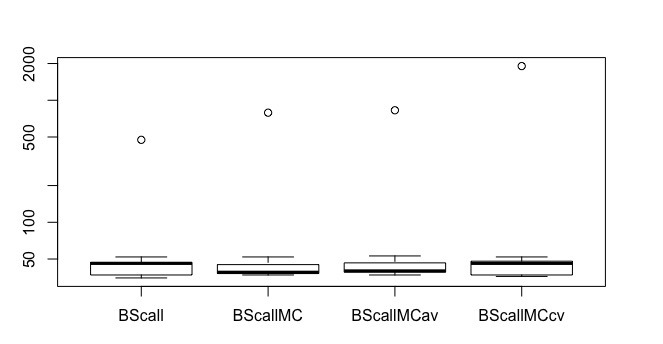
\includegraphics[width=10cm, height=8cm]{BSB}
\centering
\caption{Black-Scholes Benchmarking Boxplot}
\end{figure}







\newpage
%-------------------------
% HESTON MODEL
%-------------------------

\section{Heston model}
The aim of this chapter is to analyse and implement another option pricing model: in this specific case we deal with the Heston stochastic volatility model \cite{heston93}. This model, introduced in a paper published in 1993, builds on the aforementioned Black-Scholes model but it departs from it because it accounts for stochastic volatility of the underlying asset. \par
The constant volatility hypothesis was invalidated by empirical analysis: Black-Scholes model states that implied volatility is flat, while, in the market we observe volatility smile (smirk) in implied volatility curve.

\begin{figure}[h!]
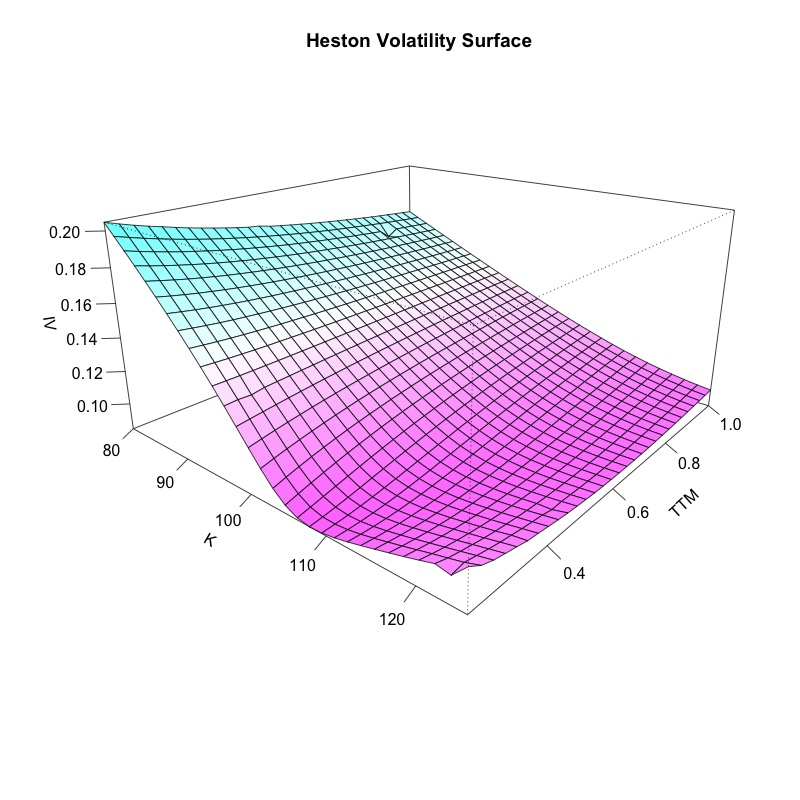
\includegraphics[width=8cm, height=8cm]{HestonVolatilitySurface}
\centering
\caption{Heston Volatility Surface}
\end{figure}

\subsection{The Model}
This model aims to derive a closed-form solution to price a European call option, by taking into account stochastic volatility. The methodology is based on characteristic functions and on differential calculus. \par
We firstly define the mathematics underneath the model. \par
Let's assume that the underlying asset price follows this process:

	\begin{equation}
		dS(t) = \mu S dt + \sqrt{v(t)} S dW_1(t)
	\end{equation}
where $W_1(t)$ is a Brownian Motion. Now, if the volatility follows an Ornstein-Uhlenbeck process, we can write the process of the volatility as follows:
	\begin{equation}
		d \sqrt{v(t)} = -\beta \sqrt{v(t)} dt + \delta dW_2(t).
	\end{equation}
	where $corr(W_1(t), W_2(t)) = \rho$.

By applying It\={o}'s calculus, it is possible to show that the process followed by $v(t)$ is:
	\begin{equation}
		dv(t) = [\delta^2 - 2 \beta v(t)]dt + 2 \delta \sqrt{v(t)} dW_2(t)
	\end{equation}
Then, by reparametrization, we can write the above equation as the well-known square-root process from Cox, Ingersoll and Ross(1985) \cite{cir} 
	\begin{equation}
		dv(t) = \kappa[\theta - v(t)] dt + \sigma \sqrt{v(t)}dW_2(t)
	\end{equation}
where $\kappa$ is the volatility mean-reversion speed, it represents how fast the volatility moves towards its long-run mean, $\theta$ is the parameter representing the long-run mean of volatility and $\sigma$ is the volatility of volatility.
Let's define the price of a discount bond:
	\begin{equation}
		P(t, t+\tau) = e^{-r \tau}
	\end{equation}
and, by doing this, we are assuming constant risk-free rate.
Now, by standard arbitrage arguments \cite{black-scholes73} we know that any asset price, $U(S, v, t)$, must satisfy the following PDE:
	\begin{equation}
	\begin{aligned}
		& \frac{1}{2} vS^" \frac{\partial^2 U}{\partial S^2} + \rho \sigma vS \frac{\partial^2 U}{\partial S \partial v} + \frac{1}{2}  \sigma^2 v  \frac{\partial^2 U}{\partial v^2} + rS \frac{\partial U}{\partial S}  \\	
		& +\{ \kappa [\theta - v(t)] - \lambda(S, v, t) \} \frac{\partial U}{\partial v} - rU +  \frac{\partial U}{\partial t} = 0
	\end{aligned}
	\end{equation}
where $\lambda(S, v, t)$ is the price of volatility risk and it is independent from the underlying asset. It is a useful parameter because it allows for change of probability measure. \par

Here, we want to define the PDE and the boundary conditions that a European Call option must satisfy.
	\begin{equation}
	\begin{aligned}
		U(S, v, T) &= Max(0, S-K),	\\
		U(0, v, t) &= 0,		\\
		\frac{\partial U}{\partial S} (\infty, v, t) &= 1,	\\
		rS \frac{\partial U}{\partial S} (S, 0, t) + \kappa \theta \frac{\partial U}{\partial v}(S, 0, t) 
		-rU(S, 0, t) + U(S, 0, t) &= 0, 	\\
		U(S, \infty, t) &= S.
	\end{aligned}
	\end{equation}
In order to be comparable to what delivered by Black-Scholes in their paper, we want to arrive to a solution of the form:
	\begin{equation}
		C(S, v, t) = SP_1 - KP_2 e^{-r \tau}
	\end{equation}  
Where $P_1$ and $P_2$ are functions of parameters: $S, K, v, t, r$.
Let's switch to logarithms. Define $x = ln(S)$. \par
Now, by plugging-in the above formula into the PDE equation it is possible to show that $P_1$ and $P_2$ must satisfy:
	\begin{equation}
	\begin{aligned}
		& \frac{1}{2} v \frac{\partial^2 P_j}{\partial x^2} + \rho \sigma v \frac{\partial^2 P_j}{\partial x \partial v} + \frac{1}{2}  \sigma^2 v  \frac{\partial^2 P_j}{\partial v^2} + (r + u_j v) \frac{\partial P_j}{\partial x}  \\	
		& +(a - b_j v)  \frac{\partial P_j}{\partial v} + \frac{\partial P_j}{\partial t} = 0
	\end{aligned}
	\end{equation}
for $j=1, 2$, where 

	\begin{equation}
	\begin{aligned}
		u_1 &= \frac{1}{2}, \\
		u_2 &= -\frac{1}{2},\\
		a &= \kappa \theta,\\
		b_1 &= \kappa + \lambda - \rho \sigma,\\
		b_2 &= \kappa+\lambda.\\
	\end{aligned}
	\end{equation}
	
	\begin{equation}
		P_j(x, v, T; ln[K]) = Pr[x(T) \leq ln[K] | x(t) = x, v(t) = v].
	\end{equation}
	
$P_j$ are the risk-neutral conditional probabilities of the options to expire in-the-money: these probabilities are not directly in closed-form. \par
But, we know that the process is exponentially affine thus, we also know that, once we get the characteristic functions, we can invert them in order to find the desired probabilities. \par
Affine processes are a class of time-homogeneous Markov processes. The logarithm of the characteristic function of the transition distribution $pt(x, �)$ of such a process is affine with respect to the initial state. \par
The coefficients defining this affine relationship are the solutions of a family of ordinary differential equations (ODEs). We classify these ODEs, called generalized Riccati equations, by their parameters, and state the precise set of admissible parameters for which there exists a unique associated regular affine process \cite{dfs}.
Here, we show the passages in order to get to a closed-form solution. \par
Assume that $x(t)$ and $v(t)$ follow the aforementioned risk-neutral process. Let's consider any twice-differentiable function $f(x, v, t)$ that is a conditional expectation of $x$ and $v$ at $T \leq t$, $g(x(T), v(T))$:

	\begin{equation} \label{eq:712}
		f(x, v, t) = \mathbb{E}[g(x(T), v(T)) | x(t) = x, v(t) = v]
	\end{equation}
	
by It\={o}:
	
	\begin{equation} \label{eq:713}
	\begin{aligned}
		df &= \bigg( \frac{1}{2} v \frac{\partial^2f}{\partial x^2} + \rho \sigma v \frac{\partial^2 f}{\partial x \partial v} + \frac{1}{2} \sigma^2 v \frac{\partial^2 f}{\partial v^2} + (r + u_j v) \frac{\partial f}{\partial x} + (a - b_j v) \frac{\partial f}{\partial v} + \frac{\partial f}{\partial t} \bigg) dt \\
		&+(r+u_j v) \frac{\partial f}{\partial x} dW_1 + (a - b_j v) \frac{\partial f}{\partial v} dW_2.
	\end{aligned}
	\end{equation}

By the Law of Iterated Expectation we know that $f$ must be a martingale: $\mathbb{E}[df] = 0$. \par
Applying this condition to \ref{eq:713} we obtain:
	
	\begin{equation}
	\begin{aligned}
		\frac{1}{2} v \frac{\partial^2 f}{\partial x^2} + \rho \sigma v \frac{\partial^2 f}{\partial x \partial v} + \frac{1}{2} \sigma^2 v \frac{\partial^2 f}{\partial v^2} + (r + u_j v) \frac{\partial f}{\partial x} + (a - b_j v) \frac{\partial f}{\partial v} + \frac{\partial f}{\partial t} = 0.
	\end{aligned}
	\end{equation}

\ref{eq:712} imposes the terminal condition $f(x, v, t) = g(x, v)$. We can solve the equation in different ways, but, for our purpose, if $g(x, v) = e^{i \phi x}$, with $i$ representing the imaginary number, then the solution is the characteristic function. In order to solve it, we guess the form:

	\begin{equation} \label{eq:715}
		f(x, v, t) = exp[C(T-t) + D(T-t) v + i \phi x].
	\end{equation}

By exploiting the linearity of the coefficient in the PDE and plugging in \ref{eq:715} into the PDE, we can reduce to two ODEs:

	\begin{equation}
	\begin {aligned}
		-\frac{1}{2} \sigma^2 \phi^2 + \rho \sigma \phi i D + \frac{1}{2} D^2 + u_j \phi i - b_j D + \frac{\partial D}{\partial t} &= 0 	\\
		r \phi i + aD + \frac{\partial C}{\partial t} &= 0 
	\end{aligned}
	\end{equation}

subjected to initial condition:
	\begin{equation}
		C(0) = 0, \hspace{1 cm} D(0) = 0.
	\end{equation}


So, define $f_1(x, v, T; \phi)$ and $f_2(x, v, T; \phi)$ characteristic functions that have to satisfy the same PDEs subjected to the final condition:
	\begin{equation}
		f_j(x, v, T; \phi) = e^{i\phi x}
	\end{equation} 
In the Heston case, the Riccati equations are defined as follows:
	\begin{equation}
	\begin{aligned}
		C(\tau; \phi) &= r \phi i \tau + \frac{a}{\sigma^2} \bigg \{ (b_j - \rho \sigma \phi i + d) \tau - 2 ln \bigg [\frac{1-ge^{d\tau}}{1-g} \bigg] \bigg\}, \\
		D(\tau; \phi) &= \frac{b_j - \rho \sigma \phi i + d}{\sigma^2} \bigg [ \frac{1-e^{d\tau}}{1-ge^{d\tau}} \bigg]
	\end{aligned}
	\end{equation}
where
	\begin{equation}
	\begin{aligned}
		g &= \frac{b_j - \rho \sigma \phi i + d}{b_j - \rho \sigma \phi i - d}, \\
		d &= \sqrt{(\rho \sigma \phi i - b_j)^2 - \sigma^2(2u_j \phi i - \phi^2)}
	\end{aligned}
	\end{equation}
Finally, as stated before, we need to invert the characteristic functions in order to get to probabilities; in order to do this, we apply the Fourier Inversion Formula \cite{heston93} \cite{dps} \cite{carrmadanfft} and use the solution of Gil-Pelaez (1951) \cite{gil} to get to the real-valued transformed characteristic function:
	\begin{equation}
		P_j(x, v, T; ln[K]) = \frac{1}{2} + \frac{1}{\pi} \int_0^\infty Re \bigg[ \frac{e^{-i \phi ln[K]} f_j(x, v, T; \phi)}{i \phi} \bigg] d\phi.  
	\end{equation}

\subsection{Features of Stochastic Volatility Model}
This section aims to analyse the effects of the stochastic volatility model: many of them are related to how the volatility evolves throughout time. \par
If we switch from physical to risk-neutral probability we are able to price options (as we state at the beginning, what we implement is a real-world approach thus, we compute values related to time-series rather than prices). In this framework, the model can be rewritten as follows:
	\begin {equation}
		dv(t) = \kappa^*[\theta^* - v(t)] dt + \sigma \sqrt{v(t)} dz_2(t)
	\end{equation}
where $\kappa^* = \kappa + \lambda$ and $\theta^* = \kappa \frac{\theta}{(\kappa + \lambda)}$.
$\theta^*$ is the variance long-run mean and $\kappa^{*}$ is the speed of mean-reversion. \par
If $\theta^*$ increases, the option price increases; $\kappa^{*}$ determines how weights are distributed between the current variance and $\theta^*$. When the movement of the mean-reversion is upward-sloping, the variance is stated to have a steady-state distribution with $mean = \theta^*$ \cite{cir}. \par
In this way, we can to find a positive feature of the Black-Scholes model: since spot returns are asymptotically Gaussian, with $variance = \theta^*$, in the long-run, the model tends to work well for long-term options. \par
It is important to keep in mind that implied variance $\theta^*$ and the "true" process variance may not be equal. We can impute this difference to the fact that we face more risk in exposing to changes in volatility.	\par
The feature to be larger or smaller of $\theta^*$ with respect to the "true" volatility depends on the sign of $\lambda$. It is possible to estimate $\theta^*$ by using value related to the option price. Or, in alternative, it is possible to estimate $\theta$ and $\kappa$ from the spot price process. \par
The parameter $\rho$ affects the skewness of spot returns distribution: when $\rho > 0$, we face high variance when the underlying asset price increases; this will cause the right tail of the density to get "fatter". On the other side, the left tail of the distribution is linked to low variance and, so, it is not modified.	\par
The parameter $\sigma$ controls the volatility of volatility. When $\sigma = 0$, the volatility is deterministic and the spot returns behave as a Gaussian distribution. In other cases we can face different effects: if the volatility is uncorrelated with spot returns, an increase in $\sigma$ increases the kurtosis of spot returns' distribution; in contrast, if we face correlation between volatility and spot returns, $\sigma$ produces skewness in the distribution.

\subsection{Implementation}
In this section we analyse the way in which the Heston option pricing model was implemented. \par
The common starting point is to price an option with built-in function. In this case, we decide to go for the $NMOF$ package that stands for Numerical Methods and Optimization in Finance. Inside this package, it is possible to find a function called  $callHestoncf$ which computes the price of a European Call under the Heston model. In order to work, it needs some parameters: $S$ is the current stock price, $X$ is the strike price, $tau$ is the time to maturity, $r$ is the risk-free rate, $q$ is the dividend rate, $v0$ is the current variance, $vT$ is the long-run variance $rho$ is the correlation between spot and variance, $k$ is the speed of mean-reversion $sigma$ is the volatility of variance. \par

\begin{lstlisting}[caption={Heston Built-In Function}]
callHestoncf(S, X, tau, r, q, v0, vT, rho, k, sigma)
\end{lstlisting}


It prices quite well from a theoretical point of view but the problem with this approach is that we just plug in values that we arbitrarily chose. \par
Then, we use the Inversion Formula, as explained in the previous section, to get a practical result starting from the theory. The following chunk of code shows how the deployment is done \cite{droberts}:

\begin{lstlisting}[caption={Heston Invesion Formula}]	
HestonInversionFormula = function(lambda, vbar, eta, rho, v0, r, tau, S0, K) {
    PIntegrand = function(u, lambda, vbar, eta, rho, v0, r, tau, S0, K, j) {
      F <- S0*exp(r*tau)
      x <- log(F/K)
      a <- lambda * vbar
      
      if (j == 1) {
        b = lambda - rho* eta
        alpha = - u^2/2 - u/2 * 1i + 1i * u
        beta = lambda - rho * eta - rho * eta * 1i * u
      } else {
        b = lambda
        alpha = - u^2/2 - u/2 * 1i
        beta = lambda - rho * eta * 1i * u
      }
      
      gamma = eta^2/2
      d = sqrt(beta^2 - 4*alpha*gamma)
      rplus = (beta + d)/(2*gamma)
      rminus = (beta - d)/(2*gamma)
      g = rminus / rplus
      
      D = rminus * (1 - exp(-d*tau))/(1-g*exp(-d*tau))
      C = lambda * (rminus * tau - 2/(eta^2) * log( (1-g*exp(-d*tau))/(1-g) ) )
      numerator = exp(C*vbar + D*v0 + 1i*u*x)
      denominator = (1i * u)
      Re(numerator/denominator)
    }    
    P = function(lambda, vbar, eta, rho, v0, r, tau, S0, K, j) {
      value = integrate(PIntegrand, lower = 0, upper = Inf,
                         lambda, vbar, eta, rho, v0, r, tau,
                         S0, K, j, subdivisions=1000)$value
      0.5 + 1/pi * value
    }
    A = S0*P(lambda, vbar, eta, rho, v0, r, tau, S0, K, 1)
    B = K*exp(-r*tau)*P(lambda, vbar, eta, rho, v0, r, tau, S0, K, 0)
    A-B
}

\end{lstlisting}


At this point, we start to develop our analysis which, in our opinion, should be, not only linked to the theory, but also coherent with the real-world framework. \par
First of all, we fit a Garch model \cite{bollerslev86} in order to get an initial condition for the parameters at the inception.\par
We build some functions useful for the pricing.\par
The following aims to simulate the volatility process, deriving from the Ornstein and Uhlenbeck process \cite{ou}.

\begin{lstlisting}[caption={OU Volatility Simulation}]
ornstein_uhlenbeck = function(T.t,nstep,nsim,theta1,theta2,theta3,x0){
dt  = T.t/nstep
Z = matrix(0, ncol = nstep, nrow = nsim) t	#Randomnorm volatility process
X = matrix(0, ncol = (1+nstep), nrow = nsim) #Volatility
X[,1] = x0
for (i in 2:(nstep+1)){ 
Z[,i-1] = rnorm(nsim, 0, sqrt(dt))
X[,i]  =  X[,i-1] + (theta1 - theta2*X[,i-1])*dt + theta3*sqrt(X[,i-1])*Z[,i-1]
}
return(OU = list(X = X, Z = Z))
}
\end{lstlisting}

The next one is useful to create the simulation of the underlying that follows the Heston process.

\begin{lstlisting}[caption = Assetpaths]
Assetpaths <- function(S0, K, sigma, T.t, r, nsim, nstep, V, Z.V){
  dt = T.t/nstep
  S = matrix(0, nsim, (1+nstep)) 
  S[,1] = rep(S0,nsim)
  for (i in 2:(nstep+1)){ 
    eps = rnorm(nsim)
    S[,i] = S[,i-1]*exp((r-0.5*V[,i-1])*dt + sqrt(V[,i-1])*(rho*Z.V[,i-1] + sqrt((1-rho^2))*dt*eps))
  }
  return(S)
}
\end{lstlisting}

Then, we apply some useful methods of Parametric Estimation \cite{iacus}.
First, let's have a glance of the theory behind the application. \par
Let's define the process that is the solution to the following SDE:
	\begin{equation}
		dX_t = (\theta_1 - \theta_2 X_t) dt + \theta_3 \sqrt{X_t} dW_t, \hspace{0.5cm} X_0 = x_0 > 0
	\end{equation}
This model can be easily reconducted to the over-described Heston model. \par
Given the condition that $2*\theta_1 > \theta_3^2$, the process is strictly positive. \par
Under this framework, the conditional density $p_\theta (t, \cdot |x)$ \cite{cir} is distributed like a non-central $\chi^2$,

	\begin{equation}
		p_\theta (t, y |x) = c e^{-u-v} \bigg( \frac{u}{v} \bigg)^{q/2} I_q(2 \sqrt{uv}),
	\end{equation}
where
	\begin{equation}
	\begin{aligned}
		c &= \frac{2 \theta_2}{\theta_3^2 (1-e^{-\theta_2t})}, \\
		q &= \frac{2 \theta_1}{\theta_3^2} - 1 \\
		u &= cxe^{-\theta_2 t}, \\
		v &= cy
	\end{aligned}
	\end{equation}

$I_q(\cdot)$ is the modified Bessel function of the first kind of order $q$,

	\begin{equation}
		I_q(x) = \sum_{k=0}^\infty \frac{x}{2}^{2\kappa+q} \frac{1}{\kappa! \Gamma(k+q+1)}
	\end{equation}

where $\Gamma (\cdot)$ is the Gamma function of the type: $\Gamma(z) = \int_0^\infty x^{z-1} e^{-x} dx$. \par
In our implementation, we use the exponential rescaled version of the Bessel Function in R because, otherwise, the function tends to explode. In order to prevent overflow, we use a modified version that computes the exponentially rescaled Bessel function using an asymptotic expansion. \par

\begin{lstlisting}[caption = Bessel Function]
expBes = function(x,nu){
  mu = 4*nu ^2
  A1 = 1
  A2 = A1 * (mu - 1) / (1 * (8*x))
  A3 = A2 * (mu - 9) / (2 * (8*x))
  A4 = A3 * (mu - 25) / (3 * (8*x))
  A5 = A4 * (mu - 49) / (4 * (8*x))
  A6 = A5 * (mu - 81) / (5 * (8*x))
  A7 = A6 * (mu -121) / (6 * (8*x))
  1/ sqrt(2*pi*x) * (A1 - A2 + A3 - A4 + A5 - A6 + A7)
}
\end{lstlisting}
This function is useful when computing SDE for the evaluation of the conditional density on real-world data. \par
Then, in order to find and calibrate the parameters, we use the log-likelihood estimation of the process. First, let's explain the function:
	\begin{equation}
		l_i(\theta) = log c - (u+v) + \frac{q}{2} log \frac{u}{v} + log I_q(2 \sqrt{uv})
	\end{equation}
In our case, by using the exponentially rescaled version, we get
	\begin{equation}
		log(e^{-x} I_q(x)) = log I_q(x) - x
	\end{equation}
Here we show the function built by starting from the log-likelihood framework. \par

\begin{lstlisting}[caption = Parameters estimation and calibration - log-likelihood]
dcCIR = function (x, t, x0 , theta , log = FALSE ){
  c = 2* theta[2] /((1 - exp(- theta[2] *t))* theta[3]^2)
  ncp = 2*c*x0*exp(- theta[2] *t)     # non centrality param of chi sq
  df = 4* theta[1] / theta[3]^2       # df of cond.prob. of chi sq con. prob
  u = c*x0* exp (- theta [2] *t)
  v = c*x
  q = 2* theta [1] / theta [3]^2 -1
  lik = ( log (c) - (u+v) + q/2 * log (v/u) + log ( expBes ( 2* sqrt (u*v), q)) + 2* sqrt (u*v))
  if(!log )
    lik = exp(lik)
  lik
}

CIR.lik = function(theta1 , theta2 , theta3 ) {
  n = length(X)
  dt = deltat(X)
  -sum(dcCIR(x=X[2: n], t=dt , x0=X[1:(n -1)] ,theta=c(theta1 , theta2 , theta3 ), log = TRUE ))
}
\end{lstlisting}

After having defined these functions, we can develop the pricing procedure as follows.	\par
We give the fitted Garch parameters values as starting condition for the parametrization
\begin{lstlisting}[caption = Heston parameters starting conditions]
	garchpara = garch(ret, order = c(1,1))
	theta2 = as.numeric(unlist(garchpara$coef[2]))                 # k
	theta1 = as.numeric(unlist(garchpara$coef[1]))*theta2          # k*long run mean
	theta3 = sqrt(2*theta1)-as.numeric(unlist(garchpara$coef[3]))  # volatility of volatility
\end{lstlisting}
\newpage
With these parameters we simulate the volatility by using the $ornstein\_uhlenbeck$ function:
\begin{lstlisting}[caption = Simulation of volatility matrix]
OU <- ornstein_uhlenbeck(T.t, nstep, nsim, theta1, theta2, theta3, x0) 
V <- OU$X #sim vola matrix
\end{lstlisting}

\begin{figure}[h]
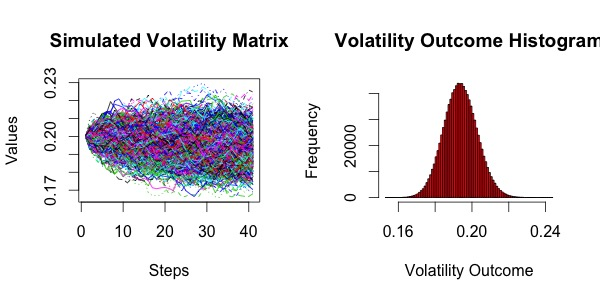
\includegraphics[scale=0.5]{simvolamatrix}
\centering
\caption{Volatility Simultion}
\end{figure}

This image represents the simulated paths and the outcomes of the volatility simulation. \par
Then, we calibrate the parameters through maximum likelihood estimation.

\begin{lstlisting}[caption = Heston parameters calibration]
X = sde.sim (X0 =.1 , model ="CIR", theta =c(theta1, theta2 , theta3), N =2500 , delta =0.1)
fit = mle(CIR.lik , start = list (theta1 =.1 , theta2 =.1 , theta3 =.3), 
          method ="L-BFGS-B", lower = c(0.001, 0.001, 0.001), upper =c(1 ,1 ,1))
long_run_mean = fit@coef[1]/fit@coef[2]
k = fit@coef[2]
sigma = fit@coef[3]
2*k*long_run_mean > sigma^2 # TRUE
OU = ornstein_uhlenbeck(T.t, nstep, nsim, theta1 <- fit@coef[1], theta2 <- fit@coef[2], theta3 <- fit@coef[3], x0)
V = OU$X
Z.V = OU$Z
\end{lstlisting}

\begin{figure}[h]
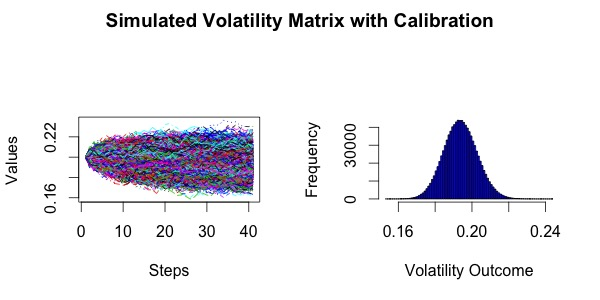
\includegraphics[scale=0.5]{simvolamatrixcalibration}
\centering
\caption{Volatility Simulation with Calibration}
\end{figure}

Here, we start the pricing procedure made by simulation.\par
We set the parameters
\begin{lstlisting}[caption = Heston pricing parameters setting]
kappa = unlist(as.numeric(fit@coef[2]))               #Mean-reversion speed
volvol = unlist(as.numeric(fit@coef[3])) 			#Volatility of volatility
theta = unlist(as.numeric(fit@coef[1]/fit@coef[2]))   #Long-term variance
\end{lstlisting}


We simulate the shocks, recall the volatility simulation and the asset path simulation and then we price via Monte Carlo.

\begin{lstlisting}[caption = Heston Option Price]
shocks <- simshocks(n =  n, horizon =  horizon, frequency =  freq,
                    method = "anti", family = 1, par =  rho)

sim.vol <- simdiff(n =  n, horizon =  horizon, frequency =  freq, model = "CIR", 
			   x0 =  V0, theta1 =  kappa*theta, theta2 =  kappa, 
			   theta3 =  volvol, eps =  shocks[[1]])

sim.price <- simdiff(n = n, horizon = horizon, frequency = freq, model = "GBM", 
			      x0 = S0, theta1 = r0, theta2 = sqrt(sim.vol), eps = shocks[[2]])
                     
S_T <- sim.price[nrow(sim.price), ]

discounted.payoff <- function(x){
  (S_T - x)*(S_T - x > 0)*exp(-r0*horizon)
}

mcprices <- sapply(strikes, function(x) mean(discounted.payoff(x)))

HestonCall <- data.frame(cbind(strikes, mcprices))
colnames(HestonCall) <- c("strikes", "mcprices")
print(HestonCall)

\end{lstlisting}

\newpage
 This is the procedure used in the implementation of the Heston model. It is not only based on merely apply the theory but also on analysing parametrisation and calibration problems.
 
The following table aims to deliver the performance, speed and accuracy, of the algorithms.

\begin{table}[h!]
\centering
\begin{tabular}{ |c|c|c|c|c|c|c|c| }
 \hline
           expr 	&	min &	lq  &	mean &		median &	uq  &	max &	neval\\
 \hline\hline
          HestonCall  &30 &31& 39.15 &  35.5& 38 & 482  & 100\\
 HestonCallClosedForm &  31& 33 &47.62&   39.5& 42 &1000 &  100\\
 \hline
\end{tabular}
\caption{Heston Benchmarking}
\label{table:Heston Speed}
\end{table}

As shown, the Monte Carlo version of the Heston formula is faster than the Inversion Formula.

\begin{figure}[h!]
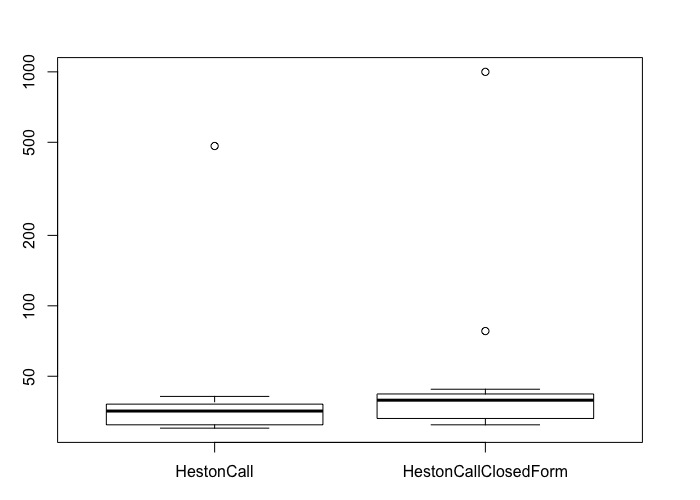
\includegraphics[width=10cm, height=6cm]{HestonBenchmarking}
\centering
\caption{Heston Benchmarking Boxplot}
\end{figure}










\newpage
%-----------------------------------------------------------------------------	
%-----------			JUMP PROCESS	  ----------------------	
%-----------------------------------------------------------------------------	
\section{Jump-Diffusion Model}
Starting from Black-Scholes model, Merton derives a more realistic view of the processes underlying stock price movements. As he stated, an issue of the BS model is that one of their assumption was that trading occurs in continuous time and also that stock prices follow a continuous sample path. It could be a good asymptotic approximation to the discrete-time solution.	\par
The validity of BS formula depends on the satisfaction of a "local" Markov property: in the short-term the stock price can change by a small amount only.	\par 
A solution to this problem is to assume a process that allows for extraordinary price changes: the jump process.

\subsection{Poisson Process}
Let $\tau$ be a random variable with density
	\begin{equation}
		f(t) = \begin{cases} \lambda e^{-\lambda t} , & t \geq 0 \\ 0, & t < 0 \end{cases}
	\end{equation}

where $\lambda > 0$ is a constant. The variable $\tau$ is exponentially distributed.
The expected value is $ \mathbb{E}\tau = \frac{1}{\lambda}$ and the $c.d.f.$ is $P\{\tau<t\} = 1 - e^{-\lambda t}, t \geq 0$. \par
A remarkable property of the exponential distribution is that after waiting a time $s$, the probability that we have to wait another  $t$ is the same as the probability of having to wait $t$ starting from $0$. This property is called memorylessness. \par

In order to build a Poisson process we need to define the sequence $\tau_1$, $\tau_2$, $...$ of independent exponential random variables, all with $\frac{1}{\lambda}$ mean. \par 
The subscript of the sequence represent the time unit at which the jump event occurs. The $\tau_k$ random variable are called interarrival times and they can be defined as:
	
	\begin{equation}
		S_n = \sum_{k = 1}^{n} \tau_k
	 \end{equation}
	 
We can define $N(t)$ as the Poisson Process with intensity $\lambda$ which counts the number of jumps that occur before time $t$:

	\begin{equation}
		f(t) = \begin{cases} 0	\hspace{0.2 cm} \text{if} \hspace{0.2 cm} 0 \leqt <S_1, \\
					      1 \hspace{0.2 cm} \text{if} \hspace{0.2 cm} S_1 \leq S_2, \\
					      \vdots	\\
					      n \hspace{0.2 cm} \text{if} \hspace{0.2 cm} S_n \leq < S_{n+1},	\\
					      \vdots
			\end{cases}
	\end{equation}
$S_n$ variable, for $n \geq 1$, has the Gamma density defined as follows:

	\begin{equation}
		g_n(s) = \frac{(\lambda s) ^{n-1}}{(n-1)!}\lambda e^{-\lambda s}
	 \end{equation}

Then, it is possible to show that the Poisson process $N(t)$ with intensity $\lambda$ has the distribution:

	\begin{equation}
		P \{ N(t) = k \} = \frac{(\lambda t)^k}{k!}e^{-\lambda t}
	 \end{equation}

Now, defined $S_n$ and the Poisson process $N_t$ with intensity $\lambda$, let's define a sequence of  independent and identically distributed random variable and call them $Y_1$, $Y_2$, $...$ with mean $\beta = \mathbf{E} Y_i$. They are mutually independent and also independent of the $N(t)$ process. We can define the compound Poisson process as follows:

	\begin{equation}
		Q(t) =  \sum_{i = 1}^{N(t)} Y_i, \hspace{0.5 cm} t \geq 0
	\end{equation}

Jumps in $Q(t)$ occurs at the same time as in $N(t)$; the difference is that in the second process we can observe only jumps where $size = 1$ whereas, in the first, they are of random size.	\par
The mean of $Q(t)$ is $\beta \lambda t$ since we have $\lambda t$ jumps in the time interval with the average jump size $\beta$.

\subsection{Properties of the Process}
	\subsubsection{Martingality}
	In a Poisson framework, $N(t)$, with intensity $\lambda$, we define the compensated Poisson process $M(t)$ as follows:
		\begin{equation}
			M(t) = N(t) - \lambda t
		\end{equation}
	Then, $M(t)$ is a martingale. \par
	Let's move to the Compound Poisson process, $Q(t)$; in this case, the compensation for the process can be defined as:
		\begin{equation}
			Q(t) - \beta \lambda t
		\end{equation}
Also the compound process is a martingale.	

	\subsubsection{Stationarity and Independence}
	Let $N(t)$ be a Poisson process with intensity $\lambda > 0$. Then the increments
		\begin{equation}
			N(t_1) - N(t_0), N(t_2) - N(t_1), ..., N(t_n) - N(t_{n-1})
		\end{equation}
	are stationary and independent, and
		\begin{equation}
			P\{N(t_{j+1}) - N(t_j) = k\} = \frac{\lambda^k (t_{j+1} - t_j)^k}{k!} e^{-\lambda(t_{j+1} - t_j)}, \hspace {0.5cm} k=0,1,...
		\end{equation}
	
	Now, let $Q(t)$ be a compound Poisson process. The increments
		\begin{equation}
			Q(t_1) - Q(t_0), Q(t_2) - Q(t_1), ..., Q(t_n) - Q(t_{n-1})
		\end{equation}

	are independent and stationary. In particular, the distribution of $Q(t_j) - Q(t_{j-1})$ is the same as the distribution of $Q(t_j - t_{j-1})$.

\subsection{Mathematical construction of a Jump Process}
\subsubsection{Process write-down}
The aim is to define the stochastic integral
	\begin{equation}
		\int_0^t \Phi(s) dX(s)
	\end{equation}
where the random variable $X$ can jump.	\par
We can define a probability space ($\Omega, \mathcal{F}, \mathcal{P}$), where the processes are $\mathcal{F}$-adapted. In addition, the integrators will be right-continuous of the form
	\begin{equation}
		X(t) = X(0) + I(t) + R(t) + J(t), \hspace{0.5 cm} X(0) \hspace{0.2cm} \mbox{is a nonrandom initial condition}.
	\end{equation}
	
The process $I(t)$ is an It\={o} integral with respect to a Brownian motion. The process $R(t)$ is a Riemann integral. $J(t)$ is an adapted, right-continuous, pure jump process with initial condition $J(0) = 0$. Here, we are denoting the jump process as $J(t)$: by doing this, we are allowing the process to be either a simple or a compound process.\par
Thus, we can write
	\begin{equation}
	\begin{aligned}
		I(t) &= \int_0^t \Gamma(s) dW(s) \\
		R(t) &= \int_0^t \Theta(s) ds \\
		X^c(t) &= X(0) + I(t) + R(t) = X(0) + \int_0^t \Gamma(s) dW(s) + \int_0^t \Theta(s) ds
	\end{aligned}
	\end{equation}
	
where $X^c(t)$ represents the continuous part of $X(t)$.

\subsubsection{Change of Measure}
For a Poisson process, the change of measure affects the intensity, whereas for a compound Poisson process it affects both intensity and the distribution jump size. \par
Once defined the Poisson process $N(t)$ and the probability space ($\Omega, \mathcal{F}, \mathcal{P}$) we can define the change of measure variable $Z(t)$ as follows:
	\begin{equation}
		Z(t) = e^{(\lambda - \widetilde\lambda)t} \bigg(\frac{\widetilde\lambda}{\lambda} \bigg)^{N(t)}
	\end{equation}
We fix $T >0 $ and we use $Z(t)$ to change to a new measure $\widetilde{P}$ under which $N(t)$ has intensity $\widetilde\lambda$.

\newpage
\subsection{Jump Process Option Pricing}
In this section we deal with pricing a European Call option when jumps occur in the underlying asset process. We can observe two different kinds of processes: in the first the asset is driven by a single Poisson process, in the second the underlying asset is driven by a Brownian motion and a Poisson process.
	
\subsubsection{Asset driven by a Poisson process}
Let's set a positive time T at which the payoff of a European call option can be written as: $V(T) = (S(T) - K)^+$. 	\par
From the theory, we also know that $\lambda > \frac{\alpha - r}{\sigma}$ in order to get rid of any possible arbitrage; thus, there exists another intensity, $\widetilde{\lambda} = \lambda - \frac{\alpha - r}{\sigma}$, which has positive value, useful as a change of measure in order to get a risk-neutral measure that can be defined as: 
	\begin{equation}
		\widetilde{P}(A) = \int_A Z(T) dP \hspace{0.5 cm} {\forall A \in \mathcal{F}}
	\end{equation}
where $Z(T) = e^{(\lambda - \widetilde{\lambda})t} (\frac{\widetilde{\lambda}}{\lambda})^{N(t)}$.
Thus, we need just to modify the GBM model for jumps; we can achieve this by allowing the stock price to be multiplied by a random factor $J$:
	\begin{equation}
		d S_t = \mu S_t dt + \sigma S_t dW_t + (J-1) S_t dN(t)
	\end{equation}
Then, by manipulating the equation through the application of risk neutrality \cite{joshi08}, we have that the $log(S(T))$ is given by:
	\begin{equation}
		\log(S_T) = \log(S_0) + \left( \mu + \frac{1}{2} \sigma^2 \right)T + \sigma \sqrt{T} N(0,1) + \sum_{j=1}^{N(T)} log J_j
	\end{equation}

Now, what we need to do is to price the option via a semi-closed form solution. \par
To get to the price, we generate random draws from a normal distribution and a Poisson distribution, and then we have to select $J_i$ values to be the size of the jumps.

\subsubsection{Asset Driven by a Brownian Motion and a Compound Poisson Process}
Given what we defined in previous sections, we can define the differential equation that models this process as follows:
		\begin{equation}
		\begin{aligned}
			dS(t) &= \alpha S(t) dt + \sigma S(t) dW(t) + S(t-) d(Q(t) - \beta \lambda t) \\
			         &= (\alpha - \beta \lambda)S(t) dt + \sigma S(t) dW(t) + S(t-)dQ(t).
		\end{aligned}
		\end{equation}
The solution to the last equation is
		\begin{equation}
			S(t) = S(0) exp \{\sigma W(t) + (\alpha - \beta \lambda - \frac{1}{2} \sigma^2)t \} \prod_{i=1}^{N(t)} (Y_i + 1).
		\end{equation}

In the practical part we deal only with the semi-closed form solution approach.

\newpage

\subsection{Implementation}
In this section we analyse the way in which jump process option pricing theory was implemented. \par
As always, the basic approach would have been to use the built-in function. In this case, we decide to go for the $NMOF$ package that stands for Numerical Methods and Optimization in Finance. Inside this package, it is possible to find a function called  $callMerton$ which computes the price of a European Call under Merton's jump-diffusion model. In order to work, it needs some parameters: $S$ is the current stock price, $X$ is the strike price, $tau$ is the time to maturity, $r$ is the risk-free rate, $q$ is the dividend rate, $\sigma$ is the variance, $\lambda$ is the jump intensity, $muJ$ is the mean size of the jumps, $vJ$ is the variance of the size of log jumps, $N$ is the number of jumps.  \par

\begin{lstlisting}[caption = Jump Built-In Function]
callMerton(S, K, T, r, 0, sigma, lambda, muJ, vJ, N, TRUE)
\end{lstlisting}

It works well as a pricing exercise: the standard approach is to draw random values from a Poisson distribution and then to compute $muJ$ and $vJ$ as mean and variance of the jump series. \par
Here, for a real-world application, as we want to develop, the problem that we faced was that, by going on the straightforward path, we can obtain positive drawings only: it means that we compute moments only from positive numbers and it is not possible to understand whether the jump is positive or negative. \par
Then, starting from the already existing function, we decide to develop an algorithm that, starting from an historical time series of a stock, and, given the fact that we can use daily prices only (so that it is not possible to observe intraday jumps), it first computes jumps and theirs moments and then prices a European call option on the over mentioned underlying assuming a jump process. \par
In order to analyse jumps in the time series, we build an algorithm that is basically a counter of non-ordinary price movements. A daily return of $+2.5\%$ is defined to be a jump of $size = 1$, $+5\%$ $size = 2$ and so on so forth; on the other side, a $-2.5\%$ is of $size = -1$, $-5\%$ $size = -2$ and so on.\par
\begin{lstlisting}[caption = Jump Counter]
jcount = NULL
jcount[1] = 0
for (i in 2:length(stockprice)){
  if (stockprice[i] > stockprice[i-1]*1.025 & stockprice[i] < stockprice[i-1]*1.05){
    jcount[i] = 1
  } else if (stockprice[i] >= stockprice[i-1]*1.5 & stockprice[i] < stockprice[i-1]*1.075 ){
    jcount[i] = 2
  } else if (stockprice[i] >= stockprice[i-1]*1.075 & stockprice[i] < stockprice[i-1]*1.10 ){
    jcount[i] = 3
  } else if (stockprice[i] >= stockprice[i-1]*1.10 & stockprice[i] < stockprice[i-1]*1.125 ){
    jcount[i] = 4
  } else if (stockprice[i] <= stockprice[i-1]*0.975 & stockprice[i] > stockprice[i-1]*0.95){
    jcount[i] = -1
  } else if (stockprice[i] <= stockprice[i-1]*0.95 & stockprice[i] > stockprice[i-1]*0.925){
    jcount[i] = -2
  } else if (stockprice[i] <= stockprice[i-1]*0.925 & stockprice[i] > stockprice[i-1]*0.875){
    jcount[i] = -3
  } else if (stockprice[i] <= stockprice[i-1]*0.875 & stockprice[i] > stockprice[i-1]*0.85){
    jcount[i] = -4
  } else if (stockprice[i] >= stockprice[i-1]*1.125 & stockprice[i] < stockprice[i-1]*1.15){
    jcount[i] = 5
  } else if (stockprice[i] >= stockprice[i-1]*1.15 & stockprice[i] < stockprice[i-1]*1.175 ){
    jcount[i] = 6
  } else if (stockprice[i] <= stockprice[i-1]*0.85 & stockprice[i] > stockprice[i-1]*0.825){
    jcount[i] = -5
  } else if (stockprice[i] <= stockprice[i-1]*0.825 & stockprice[i] > stockprice[i-1]*0.8){
    jcount[i] = -6
  } else {
    jcount[i] = 0
  }
}

muJ = mean(jcount)
logjcount = pmax(log(jcount), 0)
logjcount[is.na(logjcount)] = 0
vJ = var(logjcount)
\end{lstlisting}

\begin{figure}[h]
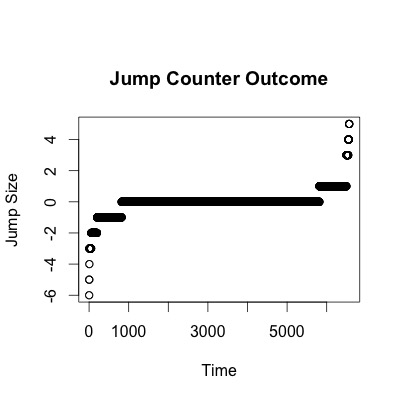
\includegraphics[scale=0.5]{jumpcounteroutcome}
\centering
\caption{Jumps in a time series}
\end{figure}
\newpage

The pricing is performed as follows: first, we price a European Call option with Black-Scholes and, by doing this, we are assuming that the underlying follows a GBM, then, we redefine volatility and the first moment by including the "jump effect" as follows \cite{merton75}:
	\begin{equation}
	\begin{aligned}
		\sigma_n &= \sigma + n \cdot \frac{vJ}{\tau} \\
 		r_n & = r - \lambda \cdot muJ + n * \frac{log(1 + muJ)}{\tau} \\
		\lambda' &= \lambda * (1 + muJ)
	\end{aligned}
	\end{equation}

Then, the European call option price is given by the following formula \cite{merton75}:
	\begin{equation}
		JumpCall = \sum^{\infty}_{n=0} \frac{e^{-\lambda ' T}(\lambda ' T)^n}{n!} BS(S_0, \sigma_n, r_n, T, K)
	\end{equation}

where $v$ is the standard deviation of the lognormal jump process and $m$ is the scale factor for jump intensity. In the appendix we give the proof of consistency of this approximation.
\begin{lstlisting}[caption = Jump option price]
#Pricing Formula
callBSM = function(S, X, tau, r, q, sigma) {
  d1 = (log(S/X) + (r - q + sigma/2) * tau)/(sqrt(sigma) * sqrt(tau))
  d2 = d1 - sqrt(sigma) * sqrt(tau)
  S * exp(-q * tau) * pnorm(d1) - X * exp(-r * tau) * pnorm(d2)
}

lambda2 = lambda * (1 + muJ)

JumpCall = 0
for (n in 0:N) {
  v_n = sigma + n * vJ/tau
  r_n = r - lambda * muJ + n * log(1 + muJ)/tau
  JumpCall = JumpCall + (exp(-lambda2 * tau) * (lambda2 * tau)^n) * callBSM(S, X, tau, r_n, q, v_n)/factorial(n)
}
JumpCall

\end{lstlisting}

Then, in order to control consistency of the application, we price the option with the built-in $callMerton$ function from $NMOF$ package and with the over mentioned procedure. \par
Once introduced the Jump, it is clear that the riskiness of the call is higher with respect to BS model; thus, on many tested underlyings the "jump call" cost more than the plain-vanilla call.


\newpage


















%-----------------------------------------------------------------------------	
%-----------			FRACTAL FRAMEWORK	  ----------------------	
%-----------------------------------------------------------------------------
\section{Fractal Framework}
The financial field is ruled by the Efficient Market Hypothesis \cite{fama}. \par
\textit{"The efficient markets hypothesis (EMH) maintains that market prices fully reflect all available information. Developed independently by Paul A. Samuelson and Eugene F. Fama in the 1960s, this idea has been applied extensively to theoretical models and empirical studies of financial securities
prices, generating considerable controversy as well as fundamental insights into the price-discovery process. The most enduring critique comes from psychologists and behavioural economists who argue that the EMH is based on counterfactual assumptions regarding human behaviour, that is, rationality."} (The New Palgrave Dictionary of Economics) \cite{lo}. \par
Starting from this theory, economists, mathematicians and psychologists (behaviouralists) tried to reconcile what the hypothesis states with what they observe in the markets.	\par
An alternative theory which attempts to overcome the "standard" hypothesis is the Fractal Market Hypotesis. \par
In this chapter we analyse this idea, its properties and we apply the theory from FMH and from Hurst analysis in order to develop a practical way to price options in the fractal framework.

\subsection{Fractal Market Hypothesis}
Fractal Market Hypotesis was proposed by Peters in 1994 \cite{peters94} and it is based on two important features of financial markets: liquidity and time horizon; it takes also into account the behaviour of investors.	\par
Markets exist to be the place in which investors can find liquidity for their trades. The idea of "fair" price as stated in the EMH is not the one taken into account here. Let's say that an extraordinary shock happens in the market: a thick-trader face a big loss in its portfolio: here, a fundamental investor can step in to bring back the market to its equilibrium. \par
Thus, the idea of fairness is that investors must share the same risk level once adjusted for their trading horizon. That's why the frequency distribution of returns look similar at different time horizon. This is a typical property of fractals: self-similarity. With self-similarity we mean that in a process, as stock prices, the parts are related to the whole. \par
To be clear, here we show a mathematical example of perfect self-similarity called Sierpinski triangle: it is a figure in which as long as we zoom in, we always observe the same pattern. 
\newpage
\begin{lstlisting}[caption = {Sierpinski Triangle}]
# Use spt package #

(abc = st(60,60))
par(mfrow = c(1,4))
plot(abc, iter=1)
plot(abc, iter=3)
plot(abc, iter=5)
plot(abc, iter=7)

\end{lstlisting}

\begin{figure}[h!]
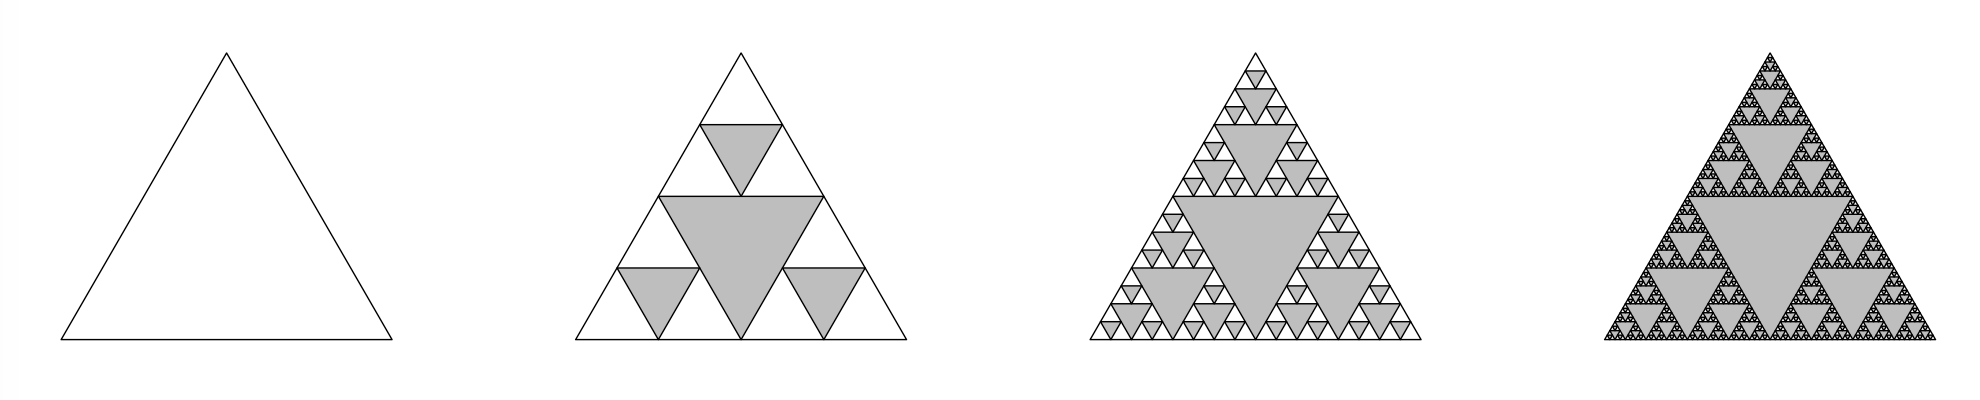
\includegraphics[scale=0.2]{sierpinskitriangle}
\centering
\caption{Sierpinski Triangle}
\end{figure}

Now, we go deep in details of what FMH proposes \cite{peters94}. \par
The market is stable when it consists of investors covering a large number of different investment horizons: this ensure liquidity. \par
This theory introduces behaviouralism into markets. It states that in the short-term, market sentiment and technical analysis are the keys to the information set; in the long run fundamental information dominates. \par
When the overall investment horizon becomes uniform (crash, financial crisis, fire sale event), the market becomes unstable. \par
Since prices reflect both technical and fundamental valuation, short-term prices tend to be more volatile than long-term. In addition it is possible to state that short-term trend are led by crowd behaviour.	\par
Trading, liquidity and short-term information dominate when the security has no tie to the economic cycle (penny stock price action, supernova pattern).




\newpage

\subsection{Fractal Analysis}
In this section we show how to implement a Rescaled Range Analysis in order to analyse a time-series and to obtain what is called Hurst Exponent $H$ which is useful for the following option pricing section.
	
\subsubsection{Measuring Memory: Hurst and R/S}
In order to create a correct framework we need to use a probability theory that is nonparametric: a very robust methodology is the one from Hurst \cite{hurst51}.	\par
The connection with fractal geometry is embedded in the \textit{Hurst exponent}: this can be approximated by plotting the $log(R/S_n)$ versus the $log(n)$ and solving for the slope through an ordinary least 	squares regression.
	\begin{equation}
		log(R/S_n) = log(c) + H \cdot log(n)
	\end{equation}
	If a system were $iid$, then $H = 0.5$.

	According to the original theory, $H=0.5$ would imply an independent process. $0 \leq H < 0.5$ means antipersistency. An antipersistent system covers less distance than a random one: for a system to cover less distance, it must reverse more often than a random one; it doesn't mean, however, that it is a mean-reverting process. $0.5 < H \leq 1$ implies a persistent time series which is characterized by long memory effect.
	
\subsubsection{How to perform and implement R/S analysis}
R/S analysis is a data-intensive, yet simple, process. \par
\begin{enumerate}
	\item We need a time series of length $M$ and then we have to convert it into a time series of length $N = M-1$ of logarithmic ratios.
		\begin{equation}
			N_i = log(M_{i+1}/M_i), \hspace{0.5 cm} i = 1, 2, 3, ..., (M+1)
		\end{equation}
		
		\begin{lstlisting}[caption = {Hurst Exponent Step 1}]
#Data
prices = stockprice
#log-returns
return = diff(log(prices))
\end{lstlisting}

\newpage
	\item Divide $N$ into $A$ contiguous subperiods of length $n$, such that $n*A = N$. The average value is defined as:
		\begin{equation}
			e_a = \frac{1}{n} \cdot \sum_{k=1}^n N_{k,a}
		\end{equation}
		where $e_a $ is the average value of $N_i$ contained in subperiod $I_a$ of length $n$.
		
	\begin{lstlisting}[caption = {Hurst Exponent Step 2}]
	
#splits
split(return, c(1:512), drop = FALSE)

#decomposition loop
k = 9
for(i in 1:k){
  h = i-1
  j = 2^h
  assign(paste("split",i,sep=""),(split(return, ceiling(seq_along(return)/(length(return)/j)))))
}

split_one = list(split1,split2,split3,split4,split5,split6,split7,split8,split9)
avg.vec = NULL
stdev.vec = NULL
for(i in 1:length(split_one)){
  avg = NULL
  stdev = NULL
  for(j in 1:length(split_one[[i]])){
    a = mean(unlist(split_one[[i]][j]))
    avg[j] = a 
    b = sd(unlist(split_one[[i]][j])) 
    stdev[j] = b
  }
  avg.vec = append(avg.vec, avg)
  stdev.vec = append(stdev.vec, stdev)
}

#errors' list
lappend = function(list, object) {
  list[[length(list)+1]] = object
  return(list)
}

list.err = list()
counter = 0

for(i in 1:length(split_one)){
  errors = list()
  for(j in 1:length(split_one[[i]])){
    a = unlist(split_one[[i]][j])-avg.vec[j+counter]
    errors[j] = list(cumsum(a))
  }
  list.err[[i]] = errors
  counter <- j + counter
}
names(vec) = NULL

	\end{lstlisting}
	
	\item Create a time series of accumulated departures ($X_{k,a}$) from the mean value for each subperiod $I_a$ as it follows:
		\begin{equation}
			X_{k,a} = \sum_{k=1}^n (N_{k,a} - e_a), \hspace{0.5 cm} k = 1, 2, 3, ..., n
		\end{equation}
		
	\begin{lstlisting}[caption = {Hurst Exponent Step 3}]
	
	#min & max error
min.vec = NULL
max.vec = NULL
for(i in 1:length(list.err)){
  min = NULL
  max = NULL
  for(j in 1:length(list.err[[i]])){
    c = min(unlist(list.err[[i]][j]))
    min[j] = c 
    d = max(unlist(list.err[[i]][j]))
    max[j] = d
  }
  min.vec = append(min.vec,min)
  max.vec = append(max.vec,max)
}

\end{lstlisting}
		
\newpage

	\item The range is defined as the maximum minus the minimum value of $X_{k,a}$ within each subperiod
		\begin{equation}
			R_{1_a} = max(X_{k, a}) - min(X_{k,a}), \hspace{0.5 cm} where \hspace{0.2 cm} 1\leq k \leq n.
		\end{equation}
	\item Compute the sample standard deviation, $S_{1_a}$ for each subperiod.
	\item Each range is now normalized by dividing by the $S_{1_a}$ corresponding to it. Therefore, the average R/S value for length $n$ is defined as
		\begin{equation}
			(R/S)_n = (1/A) \cdot \sum_{a=1}^A \frac{R_{1_a}}{S_{1_a}}
		\end{equation}
		
	\begin{lstlisting}[caption = {Hurst Exponent Step 4, 5, 6}]
#Rescaled range
rescaled = range/stdev
####
i = 0
lis = list()
for(i in 1:9){
  lis = split(avg.vec, sort(rank(avg.vec)/ 2^i))
}

# group rescaled range (R/S)

resc = list()
j = 0
split = 8
for( i in 0:split) {
  k = 2^i
  j = k + j
  resc[[i+1]] = rescaled[c(k:j)]
}

#R/S groups avg

avg.vec.resc = NULL
avg.resc = NULL
for(i in 1:length(resc)){
  h = mean(unlist(resc[[i]]))
  avg.resc[i] = h 
  avg.vec.resc[i] = rbind(avg.resc[i])
}
avg.vec.resc
	\end{lstlisting}
	
	
	\item The length $n$ is increased to the next higher value and $\frac{M-1}{n}$ is an integer. Then, repeat 1-6 until $n = \frac{M-1}{2}$. Now we can apply the following equations
		\begin{equation}
		\begin{aligned}
			(R/S)_n &= c \cdot n^H \\
			log(R/S_n) &= log(c) + H \cdot log(n)
		\end{aligned}
		\end{equation}
	
	
	\begin{lstlisting}[caption = {Hurst Exponent Step 7}]
#N
n = NULL
for(i in 1:length(split_one)){
  number = NULL
  for(j in 1:length(split_one[[i]])){
    g = length(unlist(split_one[[i]][j]))
    number[j] = g
  }
  n<-append(n,number)
}


n_0 = list()
g = 0
split = 8
for( y in 0:split) {
  u = 2^y
  g = u + g
  n_0[[y+1]] = n[c(u:g)]
}
n.vec = NULL
n.avg = NULL
for(i in 1:length(n_0)){
  h = mean(unlist(n_0[[i]]))
  n.avg[i] = h 
  
  n.vec[i] = rbind(n.avg[i])
}

n.vec


obs = log(n.vec)
R_S = log(avg.vec.resc)

#OLS
reg = (lm(R_S~obs))
summary(reg)
	
	\end{lstlisting}
	
	
By performing an OLS regression on $log(n)$ as independent variable and $log(R/S)_n$ as the dependent variable. The intercept is the estimate for $log(c)$. The slope is the estimate of the Hurst exponent $H$.
			
\begin{lstlisting}[caption = {Hurst Exponent H}]
H = as.numeric(reg$coefficients[2])
\end{lstlisting}
	\end{enumerate}

\subsection{Implementation}
Once computed the Hurst exponent $H$ for the time series, we can develop the option pricing procedure in the fractal framework by starting from the Black-Scholes model. \par
First of all, let's define some useful formulae. \par
Consider a fractional Black-Sholes market in which the stock price satisfies, under the risk-neutral measure the equation:

\begin{equation}
	dS (t) = \mu S(t)dt + \sigma S(t)dB_H (t), S (0) = S > 0, 0 \leq t \leq T 
\end{equation}

where $\mu$ an $\sigma \neq 0$  are constants and $B_H$ represents the fractional Brownian motion. \par 
In the fractional Brownian motion the increments are not independent. FBM is a continuous-time Gaussian process with $B_H(0) = 0$, $\mathbb{E}B_H(t) = 0$, for all $t$ and covariance function:

	\begin{equation}
		\mathbb{E}[B_H(t)B_H(s)] = \frac{1}{2}(|t|^{2H} + |s|^{2H} - |t-s|^{2H})
	\end{equation}
As previously stated, if $H = \frac{1}{2}$ the process is a Brownian motion, if $H > \frac{1}{2}$ the increments of the process are positively correlated, otherwise the increments of the process are negatively correlated. \par

\begin{figure}[h!]
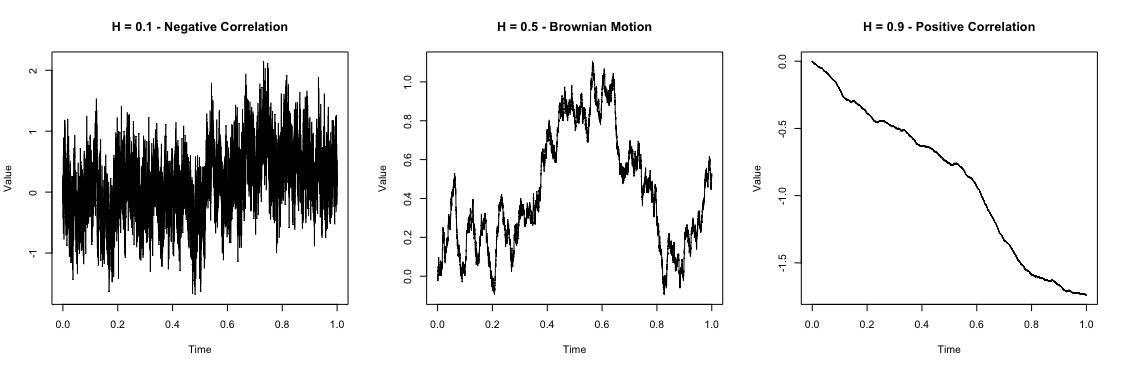
\includegraphics[scale=0.35]{FBM}
\centering
\caption{Fractional Brownian Motion}
\end{figure}


It is possible to show that this market does not have arbitrage and it is complete \cite{huoks}.
Defined the basic process, following Black-Scholes, we can price \cite{necula} a European call option as follows:

	\begin{equation}
		C(t, S(t)) = S(t) N(d_1) - K e^{-r(T-t)} N(d_2)
	\end{equation}

where

	\begin{equation}
	\begin{aligned}
		d_1 &= \frac{ln \bigg( \frac{S(t)}{K} \bigg) + r(T-t) + \frac{1}{2} \sigma^2(T^{2H} - t^{2H})}{\sigma \sqrt{T^{2H} - t^{2H}}} \\
		d_2 &= \frac{ln \bigg( \frac{S(t)}{K} \bigg) + r(T-t) - \frac{1}{2} \sigma^2(T^{2H} - t^{2H})}{\sigma \sqrt{T^{2H} - t^{2H}}}
	\end{aligned}
	\end{equation}

The fractional Brownian motion it not only depends on $(T-t)$ but also on the Hurst exponent $H$. This may be caused be the fact that FBM has longer memory than BM. In addition, it takes into account also the evolution of stock price in the period: this influence is reflected in the Hurst exponent. \par
These feature are important when we approach the market from a technical point of view: the use of Hurst analysis and fractional Brownian motion are useful in short-term horizon investment strategies. \par
In order to implement the fractal framework, we follow step-by-step the theory. \par
The following code deploy the option pricing in closed form.

\begin{lstlisting}[caption = {Fractal Option Pricing}]
FBMCall = function(S0,K,sigma,tau,r,H){
  dhat1 = (log(S0/K) + r*tau + 0.5*sigma^2*tau^(2*H))/(sigma*tau^H)
  dhat2 = dhat1 - sigma*tau^H
  FBMCall = S0 * pnorm(dhat1) - K*exp(-r*tau) * pnorm(dhat2)
  return(FBMCall)
}
\end{lstlisting}

As a proof of consistency, when we plug into the formula $H = 0.5$ we obtain the exact Black-Scholes pricing.



\afterpage{\blankpage}
\newpage
\section{Results}
The following table shows the results obtained by applying this analysis on the aforementioned stocks. \par
The values are as on 2017-02-15. \par

\begin{center}
\begin{table}[h!]
\begin{tabular}{ |c|c|c|c|c|c|c|c| }
 \hline
        Ticker    &   BSf   &  BSMC &  BSMCav  & BSMCcv  & HESTON   &  JUMP   &   FBM \\
 \hline\hline
 AAPL  & 104.8229 & 104.9152 & 104.8137 & 104.8263 & 104.9266 & 104.8571 & 104.8229 \\
 IBM  & 32.17976 & 32.13469 & 32.17897 & 32.17913 & 32.21158 & 32.18497 & 32.17976 \\
 MSFT  & 50.129 & 50.16451 & 50.13027  & 50.12755 & 50.17856 & 50.13814 & 50.129 \\
 KO  & 31.46551 & 31.48202 & 31.46594 & 31.46488 & 31.49662 & 31.47061 & 31.46551 \\
 PG  & 68.21022 & 68.24652 & 68.21117 & 68.20882 & 68.27766 & 68.22075 & 68.21022 \\
 MMM & 140.9854 & 141.0544 & 140.987 & 140.9828 & 141.1248 & 141.0077 & 140.9854 \\
 JNJ & 90.33623 & 90.38342 & 90.33744 & 90.33441 & 90.42555 & 90.35018 & 90.33623 \\
 BA  & 130.8152 & 130.8845 & 130.817 & 130.8125 & 130.9445 & 130.8383 & 130.8152 \\
 JPM  & 69.53001 & 69.57642 & 69.53157 & 69.52815 & 69.59876 & 69.54989 & 69.53001 \\
 GE  & 23.50792 & 23.52312 & 23.50841 & 23.50731 & 23.53116 & 23.51215 & 23.50792 \\
 \hline
\end{tabular}
\caption{Option Prices - Results}
\label{table: OptionPricesResults}
\end{table}
\end{center}

\begin{center}
\begin{table}[h!]
\begin{tabular}{ |c|c| }
 \hline
 BSf & Black-Scholes closed form formula \\
 BSMC & Black-Scholes Monte Carlo computation \\
 BSMCav & Black-Scholes Monte Carlo computation with antithetic variance \\
 BSMCcv & Black-Scholes Monte Carlo computation with control variates \\
 HESTON & Heston stochastic volatility model price (Our implementation) \\
 JUMP & Merton's jump diffusion model price (Our implementation) \\
 FBM & Option Pricing in the fractal Brownian motion framework \\
 \hline
\end{tabular}
\caption{Option Prices - Legend}
\label{table: OptionPricesLegend}
\end{table}
\end{center}





























\afterpage{\null\blankpage}
\newpage	

%------------------------
% CONCLUSION
%------------------------			
\section{Conclusion}
This work aimed to analyse the more famous option pricing models and to deliver a computational approach to them. \par
Starting from the mathematics and from model theory, we develop a real-world connected algorithm with the scope of finding alternative methodologies to compute option expected values. \par 
In addition we want to analyse an alternative market theory: fractal market hypothesis. \par
The aim of analysing this alternative view is to approach the market in a way different from the classical one: in this framework the focus is on price movements and patterns which relate the theory with technical analysis. \par
In our vision, this approach can be useful when we want to develop a short-term horizon option trading strategy: in this framework, an investor should take into account not only the fundamentals of a security, but also the market sentiment.	\par
Finally, the overall objective is to conclude the MSc in finance by delivering a work in which core models and applications, financial-related arguments and personal attitudes are conveyed and explained.




\afterpage{\null\blankpage}
\newpage
%------------------------
% APPENDIX
%------------------------			
\section{Appendix}
	
	%----------		PC PARITY	------------
	\subsection{Put-Call Parity}
	A European option on an underlying S pays at maturity T:
	\begin{itemize}
		\item $(S_t - K)^+$ is the payoff of a Call Option;
		\item $(K - S_t)^+$ is the payoff of a Put Option.
	\end{itemize}
	Denote the price at time $t \leq T$ of a European call option with strike price $K$ by $C_{t,T}(K)$, that of a European put option by $P_{t,T}(K)$.
	
	Put-Call Parity arises fro the mathematical identity:
		\begin{equation}	
		\begin{aligned}
			C_{t,T}(K) &= P_{t,T}(K) - K p_{t,T} + F_{t,T} p_{t,T}	\\ 	
		\end{aligned}
		\end{equation}
	
	Where $F_{t,T}$ is the Forward rate and $p_{t,T}$ is the zero-bond numeraire. 
	\par
	\underline{\textit{Proof}} \par
	
		\begin{equation}	
		\begin{aligned}
			\frac{C_{t,T}(K) - P_{t,T}(K)}{p_{t,T}} &= E^Q_t \bigg[\frac{C_{T,T}(K) - P_{T,T}(K)}{p_{T,T}} \bigg] \\
			\frac{C_{t,T}(K) - P_{t,T}(K)}{p_{t,T}} &= E^{Q_T}_t \bigg[ \frac{(S_T - K)^+ - (K-S_T)^+}{1} \bigg] \\
			\frac{C_{t,T}(K) - P_{t,T}(K)}{p_{t,T}} &= E^{Q_T}_t \bigg[ (F_{T,T}-K)^+ - (K - F_{T,T})^+ \bigg] \\
			\frac{C_{t,T}(K) - P_{t,T}(K)}{p_{t,T}} &= E^{Q_T}_t \bigg[ F_{T,T} - K \bigg] \\
			\frac{C_{t,T}(K) - P_{t,T}(K)}{p_{t,T}} &= F_{t,T} - K \\
			C_{t,T}(K) &= P_{t,T}(K) - K p_{t,T} + F_{t,T} p_{t,T}
		\end{aligned}
		\end{equation}

\newpage
%--------------Proof of Jump pricing formula -----------
\subsection{Jump Process Pricing Formula Derivation}
This section aims to derive the Merton's option pricing formula \cite{merton75}.	\par
In order to verify that the pricing formula is a solution of:
	\begin{equation}
		0 = \frac{1}{2} \sigma^2 S^2 F_{SS} + (r - \lambda k) S F_S - F_{\tau} - rF + \lambda \epsilon \{F(SY, \tau) - F(S, \tau)\}
	\end{equation}
subjected to the boundary condition:
\begin{equation}
\begin{aligned}
	F(0, \tau) &= 0, 	\\
	F(S, 0) = Max[0, S_E], 
\end{aligned}
\end{equation}
where $E$ is the exercise price of the option (previously called $K$), we can rewrite the option pricing formula  as:
	\begin{equation}
		F(S, \tau) = \sum_{n=0}^{\infty} P_n(\tau) \epsilon_n \{W(V_n, \tau; E, \sigma^2, r)\}
	\end{equation}
where $P_n(\tau) = exp [-\lambda \tau]\frac{(\lambda \tau)^n}{n!}$ and $V_n = SX_n exp[-\lambda k\tau]$. \par
By differentiating,
	\begin{equation}
	\begin{aligned}
			F_{\tau}(S, \tau) &= -\lambda F - \lambda k \sum_{n=0}^{\infty} P_n(\tau)\epsilon_n \{V_n W_1\} + \sum_{n=0}^{\infty} P_n(\tau)\epsilon_n \{W_2\} + \lambda \sum_{n=1}^{\infty} \frac{(\lambda \tau)^{n-1} e^{-\lambda \tau}}{(n-1)!} \epsilon_n \{W\} \\
			&= -\lambda F - \lambda k S F_S + \sum_{n=0}^{\infty} P_n(\tau)\epsilon_n \{W_2\} + \lambda \sum_{m=0}^{\infty} P_m(\tau) \epsilon_{m+1} \{W(V_{m+1}, \tau; E, \sigma^2, r) \} 
	\end{aligned}
	\end{equation}
where in the second line we apply a change in the summation variable: $m = n-1$.\par
We get to:
	\begin{equation}
	\begin{aligned}
		\epsilon_Y\{F(SY, \tau)\} &= \epsilon_Y \bigg[  \sum_{n=0}^{\infty} P_n(\tau) \epsilon_n \{W(V_nY, \tau; E, \sigma^2, r)\} \bigg]	\\
		&= \sum_{n=0}^{\infty} P_n(\tau) \epsilon_{n+1} \{W(V_{n+1}, \tau; E, \sigma^2, r)\}
	\end{aligned}	
	\end{equation}
Because $X_n$, $X_n+1$ and $(YX_n)$ are identically distributed.	\par
We have that:

\begin{multline}
\frac{1}{2} \sigma^2 S^2 F_{SS} + (r-\lambda k) SF_S - F_{\tau} - rF= \sum_{n=0}^{\infty} P_n(\tau) \epsilon_n \{ \frac{1}{2} \sigma^2 V-n^2 W_{11} + rV_nW_1 - W_2 - rW \} \\
- \lambda k S F_S + \lambda F + \lambda k S F_S - \lambda \sum_{n=0}^{\infty} P_m(\tau)\epsilon_{m+1} \{ W(V_{m+1}, \tau; E, \sigma^2, r) \}  	\\
&= -\lambda [\epsilon_Y \{F(SY, \tau) - F(S, \tau)] \}.
\end{multline}

W satisfies: $ \frac{1}{2} \siga^2 S^2 F_{SS} + rSF_S - rF + F_{\tau} = 0$, therefore:
	\begin{equation}
		\frac{1}{2} \siga^2 V_n^2 W_{11}+ rV_nW_1 - W_2 + rW = 0, \text{for every $n$}
	\end{equation}
$S = 0$ implies $V_n = 0$ for each $n$. In addition $W(0, \tau; E, \sigma^2, r) = 0$. \par
Thus, $F(0, \tau) = 0$ satisfies the first boundary condition. 	\par
Then, we have: 
	\begin{equation}
	\begin{aligned}
		\epsilon_n \{W(V_n, 0; E, \sigma^2, r) \} &= \epsilon_n\{Max[0, V_n-E]\} \\
		&\leq \epsilon_n \{V_n\} = S(1+k)^n.
	\end{aligned}
	\end{equation}
Therefore,
	
	\begin{equation}
	\begin{aligned}
		\lim_{\tau \to 0} \sum_{n=1}^{\infty} P_n(\tau) \epsilon_n\{W\} &\leq \lim_{\tau \to 0} \sum_{n=1}^{\infty} \frac{S e^{-\lambda \tau}[(1+k) \lambda \tau]^n}{n!}	\\
		&= \lim_{\tau \to 0} S e^{-\lambda \tau}[e^{(1+k)\lambda \tau} - 1]	\\
		&= 0.
	\end{aligned}
	\end{equation}
From this, follows:
	\begin{equation}
	\begin{aligned}
		\lim_{\tau \to 0} F(S, \tau) &= \lim_{\tau \to 0} [P_0(\tau) \epsilon_0 \{W(V_0, \tau; E, \sigma^2, r)\} \\
		&= Max[0, S-E].
	\end{aligned}
	\end{equation}
So, the pricing formula satisfies the boundary condition.








\afterpage{\null\blankpage}
\newpage
%----------------------------------
%END OF THE APPENDIX
%----------------------------------

\bibliographystyle{unsrt}
\begin{thebibliography}{9}

\bibitem{merton75}
Robert C. Merton: Option Pricing When Underlying Stock Returns Are Discontinuous, Massachusetts Institute of Technology, Cambridge, Mass. 02139, USA, 1975

\bibitem{heston93}
Steven L. Heston: A Closed-Form Solution for Options with Stochastic Volatility with Applications to Bond and Currency Options, The Review of Financial Studies 1993 Volume 6, number 2, pp. 327-343, 1993

\bibitem{black-scholes73}
Fischer Black and Myron Scholes: The Pricing of Options and Corporate Liabilities, The Journal of Political Economy, Vol. 81, No. 3 (May - Jun., 1973), pp. 637-654, The University of Chicago Press, 1973

\bibitem{shreve}
Steven E. Shreve: Stochastic Calculus for Finance II (Continuous-Time Models), Springer Finance Textbook, 2004

\bibitem{joshi08}
Mark S. Joshi: The Concepts and Practice of Mathematical Finance, Cambridge University Press, 2008

\bibitem{mandelbrot04}
Benoit B. Mandelbrot: The (Mis)Behaviour of Markets, Profile Books LTD., 2004

\bibitem{peters94}
Edgar E. Peters: Fractal Market Analysis (Applying Chaos Theory to Investment and Economics), John Wiley \& Sons INC., 1994

\bibitem{bachelier1900}
Louis J.B. Bachelier: Theory of Speculation, Annales scientifiques de l'Ecole Normale Superieure, Ser 3, 17 (1900), p. 21-86, 1900

\bibitem{bollerslev86}
Tim Bollerslev: Generalized Autoregressive Conditional Heteroskedasticity, Journal of Econometrics 31, 1986

\bibitem{iacus}
Stefano M. Iacus: Simulation and Inference for Stochastic Differential Equation, Springer, 2008

\bibitem{necula}
Ciprian Necula: Option Pricing in a Fractional Brownian Motion Environment, Academy of Economic Studies, Bucharest, 2002

\bibitem{hull}
John C. Hull: Options, Futures, and other derivatives, Prentice Hall, New York, 1997

\bibitem{hullwhite}
John C. Hull and Alan White: The pricing of options on assets with stochastic volatilities, The
Journal of Finance 42 (1987) 281-300, 1987

\bibitem{cir}
John C. Cox, Jonathan E. Ingersoll, Jr., Stephen A. Ross: A Theory of the Term Structure of Interest Rates, Econometrica, Vol. 53, No. 2 (Mar., 1985), pp. 385-407, 1985

\bibitem{dps}
Darrell Duffie, Jun Pan, Kenneth Singleton: Transform Analysis and Asset Pricing for Affine Jump-Diffusions,  Econometrica, Vol. 68, No. 6 (Nov., 2000), pp. 1343-1376, 2000

\bibitem{ou}
G. E. Uhlenbeck and L. S. Ornstein: On the Theory of the Brownian Motion, Physical Review, Vol. 36, (Sept.,1930), pp. 823-841, 1930

\bibitem{casella2010}
Christian P. Robert \& George Casella: Introducing Monte Carlo Methods with R, Springer, 2010

\bibitem{rubinstein81}
Reuven Y. Rubinstein \& Dirk P. Kroese: Simulation and the Monte Carlo Method, Wiley, New York, 1981

\bibitem{feynman}
Richard Feynman: The Feynman Lectures on Physics Vol I, Addison Wesley Longman, CalTech, 1970

\bibitem{papoulis}
A Papoulis: Brownian Movement and Markov Processes, Ch. 15 in Probability, Random Variables, and Stochastic Processes, 2nd ed. New York: McGraw-Hill, pp. 515-553, 1984.

\bibitem{weisstein}
 Eric W. Weisstein: Markov Process,  From MathWorld--A Wolfram Web Resource, http://mathworld.wolfram.com/MarkovProcess.html

\bibitem{fama}
Eugene Fama: Efficient Capital Markets: A Review of Theory and Empirical Work, The Journal of Finance, Vol. 25, No. 2, Papers and Proceedings of the Twenty-Eighth
Annual Meeting of the American Finance Association New York, N.Y. December, 28-30, 1969
(May, 1970), pp. 383-417, 1970

\bibitem{lo}
Andrew W. Lo: Efficient Market Hypothesis, From The New Palgrave Dictionary of Economics, Edited by Steven N. Durlauf and Lawrence E. Blume, 2008.

\bibitem{hurst51}
Harold E. Hurst: Long Term Storage Capacity of Reservoirs",  Transactions of the American Society of Civil Engineers, 116, 770-799, 1951.

\bibitem{dfs}
D. Duffie, D. Filipovic, W. Schachermayer: Affine Processes and Application in Finance, Stanford University, Princeton University and Vienna University of Technology, 2002.

\bibitem{dps}
Darrell Duffie, Jun Pan, Kenneth Singleton: Transform Analysis and Asset Pricing for Affine Jump-Diffusions, Econometrica, Vol. 68, No. 6 (Nov., 2000), pp. 1343-1376, 2000.

\bibitem{carrmadanfft}
Peter Carr and Dilip B. Madan: Option valuation using the fast Fourier transform, Journal of Computational Finance, 2(4):61-73, 1999.

\bibitem{gil}
J. Gil-Pelaez: Note on the inversion theorem, Biometrika 37 (1951): 481-482, 1951

\bibitem{droberts}
Dale Roberts:	\\
GitHub Repository: https://github.com/daleroberts/heston/blob/master/heston.r, 2010

\bibitem{bjork}
Thomas Bjork: Arbitrage Theory in Continuous Time, Oxford University Press, 2009

\bibitem{huoks}
Yaozhong Hu and Bernt Oksendal: Fractional White Noise Calculus and Application to Finance, Infinite dimensional analysis, quantum probability and related topics, Vol. 6, No 01: 1-32, 2000

\bibitem{necula}
Ciprian Necula: Option Pricing in a Fractional Brownian Motion Environment, Academy of Economic Studies, Bucharest, 2002


\end{thebibliography}









\end{document}